% Options for packages loaded elsewhere
\PassOptionsToPackage{unicode}{hyperref}
\PassOptionsToPackage{hyphens}{url}
%
\documentclass[
]{article}
\usepackage{amsmath,amssymb}
\usepackage{iftex}
\ifPDFTeX
  \usepackage[T1]{fontenc}
  \usepackage[utf8]{inputenc}
  \usepackage{textcomp} % provide euro and other symbols
\else % if luatex or xetex
  \usepackage{unicode-math} % this also loads fontspec
  \defaultfontfeatures{Scale=MatchLowercase}
  \defaultfontfeatures[\rmfamily]{Ligatures=TeX,Scale=1}
\fi
\usepackage{lmodern}
\ifPDFTeX\else
  % xetex/luatex font selection
\fi
% Use upquote if available, for straight quotes in verbatim environments
\IfFileExists{upquote.sty}{\usepackage{upquote}}{}
\IfFileExists{microtype.sty}{% use microtype if available
  \usepackage[]{microtype}
  \UseMicrotypeSet[protrusion]{basicmath} % disable protrusion for tt fonts
}{}
\makeatletter
\@ifundefined{KOMAClassName}{% if non-KOMA class
  \IfFileExists{parskip.sty}{%
    \usepackage{parskip}
  }{% else
    \setlength{\parindent}{0pt}
    \setlength{\parskip}{6pt plus 2pt minus 1pt}}
}{% if KOMA class
  \KOMAoptions{parskip=half}}
\makeatother
\usepackage{xcolor}
\usepackage[margin=1in]{geometry}
\usepackage{graphicx}
\makeatletter
\def\maxwidth{\ifdim\Gin@nat@width>\linewidth\linewidth\else\Gin@nat@width\fi}
\def\maxheight{\ifdim\Gin@nat@height>\textheight\textheight\else\Gin@nat@height\fi}
\makeatother
% Scale images if necessary, so that they will not overflow the page
% margins by default, and it is still possible to overwrite the defaults
% using explicit options in \includegraphics[width, height, ...]{}
\setkeys{Gin}{width=\maxwidth,height=\maxheight,keepaspectratio}
% Set default figure placement to htbp
\makeatletter
\def\fps@figure{htbp}
\makeatother
\setlength{\emergencystretch}{3em} % prevent overfull lines
\providecommand{\tightlist}{%
  \setlength{\itemsep}{0pt}\setlength{\parskip}{0pt}}
\setcounter{secnumdepth}{-\maxdimen} % remove section numbering

%\newcommand{\beginsupplement}{%
%        \setcounter{table}{0}
%        \renewcommand{\thetable}{\arabic{table}}%
%        \setcounter{figure}{0}
%        \renewcommand{\thefigure}{\arabic{figure}}%
%     }

\newcommand{\beginsupplement}{
	\renewcommand{\figurename}{Supplementary Figure}
	\setcounter{figure}{0}
}

\usepackage{xr}
\externaldocument{Supplementary_File1}

\usepackage{lineno}
\linenumbers

\usepackage[compress, super]{natbib}

\usepackage{setspace} \doublespacing

\usepackage{siunitx}

\usepackage[utf8]{inputenc}
\usepackage{amsmath}
\usepackage{algorithm}
\usepackage{algpseudocode}

\algrenewcommand\algorithmicrequire{\textbf{Input:}}
\algrenewcommand\algorithmicensure{\textbf{Output:}}
\ifLuaTeX
  \usepackage{selnolig}  % disable illegal ligatures
\fi
\IfFileExists{bookmark.sty}{\usepackage{bookmark}}{\usepackage{hyperref}}
\IfFileExists{xurl.sty}{\usepackage{xurl}}{} % add URL line breaks if available
\urlstyle{same}
\hypersetup{
  pdftitle={Transcripts with high distal heritability mediate genetic effects on complex metabolic traits},
  hidelinks,
  pdfcreator={LaTeX via pandoc}}

\title{Transcripts with high distal heritability mediate genetic effects
on complex metabolic traits}
\author{}
\date{\vspace{-2.5em}}

\begin{document}
\maketitle

Anna L. Tyler\textsuperscript{1}, J. Matthew Mahoney\textsuperscript{1},
Mark P. Keller\textsuperscript{2}, Candice N. Baker\textsuperscript{1},
Margaret Gaca\textsuperscript{1}, Anuj Srivastava\textsuperscript{1},
Isabela Gerdes Gyuricza\textsuperscript{1}, Madeleine J.
Braun\textsuperscript{1}, Nadia A. Rosenthal\textsuperscript{1}, Alan D.
Attie\textsuperscript{2}, Gary A. Churchill\textsuperscript{1} and
Gregory W. Carter\textsuperscript{1}

\textsuperscript{1}The Jackson Laboratory, Bar Harbor, Maine, USA.
\textsuperscript{2}University of Wisconsin-Madison, Biochemistry
Department, Madison, Wisconsin, USA.

\subsection{Abstract}\label{abstract}

Although many genes are subject to local regulation, recent evidence
suggests that complex distal regulation may be more important in
mediating phenotypic variability. To assess the role of distal gene
regulation in complex traits, we combine multi-tissue transcriptomes
with physiological outcomes to model diet-induced obesity and metabolic
disease in a population of Diversity Outbred mice. Using a novel
high-dimensional mediation analysis, we identify a composite
transcriptome signature that summarizes genetic effects on gene
expression and explains 30\% of the variation across all metabolic
traits. The signature is heritable, interpretable in biological terms,
and predicts obesity status from gene expression in an independently
derived mouse cohort and multiple human studies. Transcripts
contributing most strongly to this composite mediator frequently have
complex, distal regulation distributed throughout the genome. These
results suggest that trait-relevant variation in transcription is
largely distally regulated, but is nonetheless identifiable,
interpretable, and translatable across species.

\subsection{Introduction}\label{introduction}

Evidence from genome-wide association studies (GWAS) suggests that most
heritable variation in complex traits is mediated through regulation of
gene expression. The majority of trait-associated variants lie in gene
regulatory regions
\cite{pmid22955828, pmid25363779, pmid21617055, pmid19474294, 
pmid24702953, pmid24316577, pmid27126046}, suggesting a relatively
simple causal model in which a variant alters the homeostatic expression
level of a nearby (local) gene which, in turn, alters a trait.
Statistical methods such as transcriptome-wide association studies
(TWAS) \cite{pmid33020666, pmid26258848, pmid27019110, pmid26854917} and
summary data-based Mendelian randomization (SMR) \cite{pmid27019110}
have used this idea to identify genes associated with multiple disease
traits \cite{pmid29567659, 
pmid35533209,  pmid27309819, pmid30950127}. However, despite the great
promise of these methods, explaining trait effects with local gene
regulation has been more difficult than initially assumed
\cite{pmid32912663, pmid36515579}. Although trait-associated variants
typically lie in non-coding, regulatory regions, these variants often
have no detectable effects on gene expression \cite{pmid32912663} and
tend not to co-localize with expression quantitative trait loci (eQTLs)
\cite{pmid36515579, pmid37857933}. These observations suggest that the
relationship among genetic variants, gene expression, and organism-level
traits is more complex than the simple, local model.

In recent years the conversation around the genetic architecture of
common disease traits has been addressing this complexity, and there is
increased interest in more distant (distal) genetic effects as potential
drivers of trait variation \cite{pmid37857933, 
pmid32424349, pmid32831138, pmid30950127, pmid24013639}. In general,
distal effects are defined as being greater than 4 or 5Mb away from the
transcription start site of a given gene. We use the terms local and
distal rather than \textit{cis} and \textit{trans} because \textit{cis}
and \textit{trans} have specific biochemical meanings
\cite{pmid18597885}, whereas local and distal are defined only by
genomic position. The importance of distal genetic effects is proposed
in the omnigenic model, which posits that trait-driving genes are
cumulatively influenced by many distal variants. In this view, the
heritable transcriptomic signatures driving clinical traits are an
emergent state arising from the myriad molecular interactions defining
and constraining gene expression. Consistent with this view, it has been
suggested that part of the difficulty in explaining trait variation
through local eQTLs may arise in part because gene expression is not
measured in the appropriate cell types \cite{pmid32912663}, or cell
states \cite{pmid35545678}, and thus local eQTLs influencing traits
cannot be detected in bulk tissue samples. This context dependence
emphasizes the essential role of complex regulatory and tissue networks
in mediating variant effects. The mechanistic dissection of complex
traits in this model is more challenging because it requires addressing
network-mediated effects that are weaker and greater in number. However,
the comparative importance of distal effects over local effects is
currently only conjectured and challenging to address in human
populations.

To assess the role of wide-spread distal gene regulation in the genetic
architecture of complex traits, we used genetically diverse mice as a
model system. In mice we can obtain simultaneous measurements of the
genome, transcriptome, and phenome in all individuals. We used
diet-induced obesity and metabolic disease as an archetypal example of a
complex trait. In humans, these phenotypes are genetically complex with
hundreds of variants mapped through GWAS \cite{pmid36350656, 
pmid34556834} that are known to act through multiple tissues
\cite{pmid28089486, pmid10889786}. Likewise in mice, metabolic traits
are also genetically complex \cite{pmid31343992} and synteny analysis
implicates a high degree of concordance in the genetic architecture
between species \cite{pmid31343992, pmid29567659}. Furthermore, in
contrast to humans, in mice we have access to multiple disease-relevant
tissues in the same individuals with sufficient numbers for adequate
statistical power.

We generated two complementary data sets: a discovery data set in a
large population of Diversity Outbred (DO) mice \cite{pmid22892839}, and
an independent validation data set derived by crossing inbred strains
from the Collaborative Cross (CC) recombinant inbred lines
\cite{pmid18716833} to form CC recombinant inbred intercross (CC-RIX)
mice. Both populations were maintained on a high-fat, high-sugar diet to
model diet-induced obesity and metabolic disease \cite{pmid29567659}.

The DO population and CC recombinant inbred lines were derived from the
same eight inbred founder strains: five classical lab strains and three
strains more recently derived from wild mice \cite{pmid22892839},
representing three subspecies and capturing 90\% of the known variation
in laboratory mice \cite{pmid31133439}. The DO mice are maintained with
a breeding scheme that ensures equal contributions from each founder
across the genome thus rendering almost the whole genome visible to
genetic inquiry and maximizing power to detect eQTLs
\cite{pmid22892839}. The CC mice were initially intercrossed to
recombine the genomes from all eight founders, and then inbred for at
least 20 generations to create recombinant inbred lines
\cite{pmid18716833, pmid21411855, 
pmid31133439}. Because these two populations have common ancestral
haplotypes but highly distinct kinship structure, we could directly and
unambiguously compare the local genetic effects on gene expression at
the whole-transcriptome level while varying the population structure
driving distal regulation.

In the DO population, we paired clinically relevant metabolic traits,
including body weight and plasma levels of insulin, glucose and lipids
\cite{pmid29567659}, with transcriptome-wide gene expression in four
tissues related to metabolic disease: adipose tissue, pancreatic islets,
liver, and skeletal muscle. We measured similar metabolic traits in a
CC-RIX population and gene expression from three of the four tissues
used in the DO: adipose tissue, liver, and skeletal muscle. Measuring
gene expression in multiple tissues is critical to adequately assess the
extent to which local gene regulation varies across the tissues and
whether such variability might account for previous failed attempts to
identify trait-relevant local eQTLs. The CC-RIX carry the same founder
alleles as the DO. Thus, local gene regulation is expected to match
between the populations. However, because the alleles are recombined
throughout the genome, distal effects are expected to vary from those in
the DO, allowing us to directly assess the role of distal gene
regulation in driving trait-associated transcript variation. To
mechanistically dissect distal effects on metabolic disease, we
developed a novel dimension reduction framework called high-dimensional
mediation analysis (HDMA) to identify the heritable transcriptomic
signatures driving trait variation, which we compared between mouse
populations and to human data sets with measured adipose gene
expression. Together, these data enable a comprehensive view into the
genetic architecture of metabolic disease.

\subsection{Results}\label{results}

\subsubsection{Genetic variation contributed to wide phenotypic
variation}\label{genetic-variation-contributed-to-wide-phenotypic-variation}

Although the environment was consistent across the DO mice, the genetic
diversity present in this population resulted in widely varying
distributions across physiological measurements (Fig.
\ref{fig:trait_overview}). For example, body weights of adult
individuals varied from less than the average adult C57BL/6J (B6) body
weight to several times the body weight of a B6 adult in both sexes
(Males: 18.5 - 69.1g, Females: 16.0 - 54.8g) (Fig.
\ref{fig:trait_overview}A). Fasting blood glucose (FBG) also varied
considerably (Fig. \ref{fig:trait_overview}B), although few of the
animals had FBG levels that would indicate pre-diabetes (19 animals,
3.8\%), or diabetes (7 animals, 1.4\%) according to previously developed
cutoffs (pre-diabetes: FBG \(\geq\) 250 mg/dL, diabetes: FBG \(\geq\)
300, mg/dL) \cite{pmid17018838}. Males had higher FBG than females on
average (Fig. \ref{fig:trait_overview}C) as has been observed before
suggesting either that males were more susceptible to metabolic disease
on the high-fat, high-sugar (HFHS) diet, or that males and females may
require different thresholds for pre-diabetes and diabetes.

Body weight was strongly positively correlated with food consumption
(Fig. \ref{fig:trait_overview}D \(R^2 =\) 0.51, \(p<\)
\ensuremath{2.2\times 10^{-16}}) and FBG (Fig.
\ref{fig:trait_overview}E, \(R^2=\) 0.21, \(p <\)
\ensuremath{2.2\times 10^{-16}}) suggesting a link between behavioral
factors and metabolic disease. However, the heritability of this trait
and others (Fig. \ref{fig:trait_overview}F) indicates that genetics
contribute substantially to correlates of metabolic disease in this
population.

The trait correlations (Fig. \ref{fig:trait_overview}G) showed that most
of the metabolic trait pairs were only modestly correlated, which, in
conjunction with the trait decomposition (Supplementary Figure
\ref{fig:trait_decomp}), suggests complex relationships among the
measured traits and a broad sampling of multiple heritable aspects of
metabolic disease including overall body weight, glucose homeostasis,
and pancreatic function.

\subsubsection{Distal Heritability Correlated with Phenotype
Relevance}\label{distal-heritability-correlated-with-phenotype-relevance}

It is widely assumed that variation in traits is mediated through local
regulation of gene expression. To test this assumption, we measured
transcriptome-wide gene expression in four tissues--adipose, liver,
pancreatic islet, and skeletal muscle--in the DO cohort. (Basic results
from a standard eQTL analysis \cite{pmid30591514} (Methods) are
available in Supplementary Figure \ref{fig:eQTL}). We estimated the
local genetic contribution to each transcript as the variance explained
by the haplotype probabilities at the genetic marker closest to the gene
transcription start site. We estimated the distal heritability as the
heritability of the residuals after local haplotype had been accounted
for (Methods). Importantly, this estimate was not based on distal eQTL,
but rather the unlocalized contribution of the genome after removing the
local genetic effect.

Overall, local and distal genetic factors contributed approximately
equally to transcript abundance. In all tissues, both local and distal
factors explained between 8 and 17\% of the variance in the median
transcript (Fig, \ref{fig:motivation}A). This 50\% contribution of local
genetic variation to transcript abundance contrasts with findings in
humans in which local variants have been found to explain only 20-30\%
of total heritability, while distal effects explain the remaining
70-80\%\cite{pmid31558840, pmid21383966}. This discrepancy may arise due
to the high degree of linkage disequilibrium in the DO mice compared to
human populations and to the high degree of confidence with which we can
estimate ancestral haplotypes in this population. At each position in
the mice we can estimate ancestral haplotype with a high degree of
accuracy. Haplotype at any given genetic marker captures genomic
information from a relatively large genomic region surrounding each
marker. In contrast, there is a much higher degree of recombination in
human populations and ancestral haplotypes are more numerous and more
difficult to estimate than in the mice. Thus in the mice, each marker
may capture more local regulatory variation than SNPs or estimated
haplotypes capture in humans. It has been found that transcripts with
muliple local eQTL have higher local heritability than transcripts with
single local eQTL\cite{pmid25010687}. Because of the high diversity in
the DO and the high rates of linkage disequilibrium, it is possible that
there are more local variants regulating transcription creating a
proportionally larger effect of local regulation.

To assess the importance of genetic regulation of transcript levels to
clinical traits, we compared the local and distal heritabilities of
transcripts to their trait relevance. We defined trait relevance for a
transcript as its maximum absolute Spearman correlation coefficient
(\(\rho\)) across all traits (Methods). The local heritability of
transcripts was negatively associated with their trait relevance (Fig.
\ref{fig:motivation}B), suggesting that the more local genotype
influenced transcript abundance, the less effect this variation had on
the measured traits. Conversely, the distal heritability of transcripts
was positively associated with trait relevance (Fig.
\ref{fig:motivation}C). That is, transcripts that were more highly
correlated with the measured traits tended to be distally, rather than
locally, heritable. Importantly, this pattern was consistent across all
tissues. This finding is also consistent with previous observations that
transcripts with low local heritability explain more expression-mediated
disease heritability than transcripts with high local heritability
\cite{pmid32424349}. However, the positive relationship between trait
correlation and distal heritability demonstrated further that there are
diffuse genetic effects throughout the genome converging on
trait-related transcripts.

\subsubsection{High-Dimensional Mediation Analysis identified a
high-heritability composite trait that was mediated by a composite
transcript}\label{high-dimensional-mediation-analysis-identified-a-high-heritability-composite-trait-that-was-mediated-by-a-composite-transcript}

The above univariate analyses establish the importance of distal
heritability for trait-relevant transcripts. However, the number of
transcripts dramatically exceeds the number of phenotypes. Thus, we
expect the heritable, trait-relevant transcripts to be highly correlated
and organized according to coherent, biological processes representing
the mediating endophenotypes driving clinical trait variation. To
identify these endophenotypes in a theoretically principled way, we
developed a novel dimension-reduction technique, high-dimension
mediation analysis (HDMA), that uses the theory of causal graphical
models to identify a transcriptomic signature that is simultaneously 1)
highly heritable, 2) strongly correlated to the measured phenotypes, and
3) conforms to the causal mediation hypothesis (Fig.
\ref{fig:workflow}). In HDMA, we first use a linear mapping called
kernelization to dimension-reduce the genome, transcriptome, and phenome
to kernel matrices \(G_K\), \(T_K\) and \(P_K\) respectively, which each
have the dimensions \(n\) by \(n\) where \(n\) is the number of
individuals (Methods). These kernel matrices describe the relationships
among the individual mice in genome space, transcriptome space, and
phenome space and ensure that these three omic spaces have the same
dimensions, and thus the same weight in the analysis. If not
dimension-reduced, the transcriptome would outweigh the phenome in the
model. We then projected these \(n \times n\)-dimensional kernel
matrices onto one-dimensional scores--a composite genome score
(\(G_C\)), a composite transcriptome score (\(T_C\)), and a composite
phenome score (\(P_C\))--and used the univariate theory of mediation to
constrain these projections to satisfy the hypotheses of perfect
mediation, namely that upon controlling for the transcriptomic score,
the genome score is uncorrelated to the phenome score. A complete
mathematical derivation and implementation details for HDMA are
available in the Methods.

Using HDMA we identifed the major axis of variation in the transcriptome
that was consistent with mediating the effects of the genome on
metabolic traits (Fig \ref{fig:workflow}). Fig. \ref{fig:workflow}A
shows the partial correlations (\(\rho\)) between the pairs of these
composite vectors. The partial correlation between \(G_C\) and \(T_C\)
was 0.42, and the partial correlation between \(T_C\) and \(P_C\) was
0.78. However, when the transcriptome was taken into account, the
partial correlation between \(G_C\) and \(P_C\) was effectively zero
(0.039). \(P_C\) captured 30\% of the overall trait variance, and its
estimated heritability was 0.71 \(\pm\) 0.084, which was higher than any
of the measured traits (Fig. \ref{fig:trait_overview}F). Thus, HDMA
identified a maximally heritable metabolic composite trait and a highly
heritable component of the transcriptome that are correlated as expected
in the perfect mediation model.

As discussed in the Methods, HDMA is related to a generalized form of
canonical correlation analysis (CCA). Standard CCA is prone to
over-fitting because in any two large matrices it can be trivial to
identify highly correlated composite vectors \cite{pmid38383808}. To
assess whether our implementation of HDMA was similarly prone to
over-fitting in a high-dimensional space, we performed permutation
testing. We permuted the individual labels on the transcriptome matrix
10,000 times and recalculated the path coefficient, which is the
correlation of \(G_C\) and \(T_C\) multiplied by the correlation of
\(T_C\) and \(P_C\). This represents the strength of the path from
\(G_C\) to \(P_C\) that is putatively mediated through \(T_C\). The
permutations preserved the correlation between the genome and phenome,
but broke the correlations between the genome and the transcriptome, as
well as between the transcriptome and the phenome. We could thus test
whether, given a random transcriptome, HDMA would overfit and identify
apparently mediating transcriptomic signatures in random data. The null
distribution of the path coefficient is shown in Fig.
\ref{fig:workflow}B, and the observed path coefficient from the original
data is indicated by a red arrow. The observed path coefficient was well
outside the null distribution generated by permutations
(\(p < 10^{-16}\)). Fig. \ref{fig:workflow}C illustrates this
observation in more detail. Although we identified high correlations
between \(G_C\) and \(T_C\), and modest correlations between \(T_C\) and
\(P_C\) in the null data (Fig \ref{fig:workflow}C), these two values
could not be maximized simultaneously in the null data. In contrast, the
red dot shows that in the real data both the \(G_C\)-\(T_C\) correlation
and the \(T_C\)-\(P_C\) correlation could be maximized simultaneously
suggesting that the path from genotype to phenotype through the
transcriptome is highly non-trivial and identifiable in this case.

To test whether the presence of local eQTLs affected the result, we
generated two additional transcriptomic kernel matrices. To generate a
distal kernel we regressed out the effect of local haplotype from each
transcript and calculated the kernel from only distally regulated
transcription. We generated a local kernel using only locally determined
gene expression and a distal kernel using only distally determined gene
expression, i.e.~the effects of local haplotype were regressed out. The
path coefficient identified using the local kernel was not significantly
different from the null (Fig. \ref{fig:workflow}B), suggesting that
locally determined gene expression does not mediate the effects of the
genome on the phenome. In contrast, the path coefficient identified
using the distal kernel, was highly significant and indistinguishable
from that identified using the full transcriptome.

Further, the \(G_C\)-\(T_C\) and \(T_C\)-\(P_C\) correlations derived
from the distal kernal were indistinguishable from those derived from
the original transcriptomic kernel. In contrast, the \(G_C\)-\(T_C\)
correlation derived with the local kernel was high, reflecting the fact
that the local transcriptomic kernel was derived directly from local
haplotypes. The \(T_C\)-\(P_C\) correlation, however, was low (0.14),
suggesting that the these locally derived transcripts were not highly
related to phenotype. In other words, mice that shared many local eQTL
were not highly similar in trait space. Taken together, these results
suggest that composite vectors derived from the measured transcriptomic
kernel represent genetically determined variation in phenotype that is
mediated through genetically determined variation in transcription, and
that this genetically deremined variation in transcription is largely
driven by distal factors.

\subsubsection{Body weight and insulin resistance were highly
represented in the expression-mediated composite
trait}\label{body-weight-and-insulin-resistance-were-highly-represented-in-the-expression-mediated-composite-trait}

Each composite score is a weighted combination of the measured
variables. The magnitude and sign of the weights, called loadings,
correspond to the relative importance and directionality of each
variable in the composite score. The loadings of each measured trait
onto \(P_C\) indicate how much each contributed to the composite
phenotype. Body weight contributed the most (Fig.
\ref{fig:interpretation}), followed by homeostatic insulin resistance
(HOMA\_IR) and fasting plasma insulin levels (Insulin\_Fasting). We can
thus interpret \(P_C\) as an index of metabolic disease (Fig.
\ref{fig:interpretation}B). Individuals with high values of \(P_C\) have
a higher metabolic disease index (MDI) and greater metabolic disease,
including higher body weight and higher insulin resistance. We refer to
\(P_C\) as MDI going forward. Traits contributing the least to MDI were
measures of cholesterol and pancreas composition. Thus, when we
interpret the transcriptomic signature identified by HDMA, we are
explaining primarily the putative transcriptional mediation of body
weight and insulin resistance, as opposed to cholesterol measurements.

\subsubsection{High-loading transcripts had low local heritability, high
distal heritability, and were linked mechanistically to
obesity}\label{high-loading-transcripts-had-low-local-heritability-high-distal-heritability-and-were-linked-mechanistically-to-obesity}

We interpreted large loadings onto transcripts as indicating strong
mediation of the effect of genetics on MDI. Large positive loadings
indicate that higher expression was associated with a higher MDI
(i.e.~higher risk of obesity and metabolic disease on the HFHS diet)
(Fig. \ref{fig:interpretation}C-D). Conversely, large negative loadings
indicate that high expression of these transcripts was associated with a
lower MDI (i.e.~lower risk of obesity and metabolic disease on the HFHS
diet) (Fig. \ref{fig:interpretation}C-D). Fig. \ref{fig:interpretation}D
compares the observed transcript loading distributions to null
distributions and indicates how many transcripts in each tissue had
large positive and negative loadings. A direct comparison of the tissues
can be seen in Supplementary Figure
\ref{fig:transcript_loading_comparison}. We used gene set enrichment
analysis (GSEA) \cite{fgsea, 
pmid16199517} to look for biological processes and pathways that were
enriched at the top and bottom of this list (Methods).

In adipose tissue, both GO processes and KEGG pathway enrichments
pointed to an axis of inflammation and metabolism (Figs.
\ref{fig:top_enrich_kegg} and \ref{fig:top_enrich_go}). GO terms and
KEGG pathways associated with inflammation were positively associated
with MDI, indicating that increased expression in inflammatory pathways
was associated with a higher burden of disease. It is well established
that adipose tissue in obese individuals is inflamed and infiltrated by
macrophages \cite{pmid19133410, 
pmid28955384, pmid28912810, pmid28901330, pmid24969772}, and the results
here suggest that this may be a dominant heritable component of
metabolic disease.

The strongest negative enrichments in adipose tissue were related to
mitochondial activity in general, and thermogenesis in particular (Figs.
\ref{fig:top_enrich_kegg} and \ref{fig:top_enrich_go}). Genes in the
KEGG oxidative phosphorylation pathway were almost universally
negatively loaded in adipose tissue, suggesting that increased
expression of these genes was associated with reduced MDI (Supplementary
Figure \ref{fig:oxPhos}). Consistent with this observation, it has been
shown previously that mouse strains with greater thermogenic potential
are also less susceptible to obesity on an obesigenic diet
\cite{pmid18492779}.

Transcripts associated with the citric acid cycle as well as the
catabolism of the branched-chain amino acids (valine, leuceine, and
isoleucine) were strongly enriched with negative loadings in adipose
tissue (Supplementary Figures \ref{fig:top_enrich_kegg},
\ref{fig:TCA_cycle} and \ref{fig:bcaa_degrataion}). Expression of genes
in both pathways (for which there is some overlap) has been previously
associated with insulin sensitivity \cite{pmid29567659, 
pmid22560213, pmid19841271}, suggesting that heritable variation in
regulation of these pathways may influence risk of insulin resistance.

Looking at the 10 most positively and negatively loaded transcripts from
each tissue, it is apparent that transcripts in the adipose tissue had
the largest loadings, both positive and negative (Fig.
\ref{fig:loading_heritability}A bar plot). This suggests that much of
the effect of genetics on body weight and insulin reisistance is
mediated through gene expression in adipose tissue. This finding does
not speak to the relative importance of tissues not included in this
study, such as brain, in which transcriptional variation may mediate a
large portion of the genetic effect on obesity. The strongest loadings
in liver and pancreas were comparable, and those in skeletal muscle were
the weakest (Fig. \ref{fig:loading_heritability}A), suggesting that less
of the genetic effects were mediated through transcription in skeletal
muscle. As expected, heritability analysis showed that transcripts with
the largest loadings had higher distal heritability than local
heritability (Fig. \ref{fig:loading_heritability}A heat map and box
plot). We also performed TWAS in this population by imputing transcript
levels for each gene based on local genotype only and correlating the
imputed transcript levels with each trait. In contrast to HDMA, the TWAS
procedure tended to nominate transcripts with lower loadings (Fig.
\ref{fig:loading_heritability}B), higher local heritability and lower
distal heritability. Finally, we focused on transcripts with the highest
local heritability in each tissue (Fig.
\ref{fig:loading_heritability}C). This procedure selected transcripts
with low loadings on average, consistent with our findings above (Fig.
\ref{fig:motivation}B).

We performed a literature search for the genes in each of these groups
along with the terms diabetes, obesity, and the name of the expressing
tissue to determine whether any of these genes had previous associations
with metabolic disease in the literature (Methods). Multiple genes in
each group had been previously associated with obesity and diabetes
(Fig. \ref{fig:loading_heritability} bolded gene names). Genes with high
loadings were most highly enriched for previous literature support. They
were 2.2 times more likely than TWAS hits and 4 times more likely than
genes with high local heritability to be previously associated with
obesity or diabetes.

\subsubsection{Tissue-specific transriptional programs were associated
with metabolic
traits}\label{tissue-specific-transriptional-programs-were-associated-with-metabolic-traits}

Clustering of transcripts with top loadings in each tissue showed
tissue-specific functional modules associated with obesity and insulin
resistance (Fig. \ref{fig:toa}A) (Methods). The clustering highlights
the importance of immune activation particularly in adipose tissue. The
mitosis cluster had large positive loadings in three of the four tissues
potentially suggesting system-wide proliferation of immune cells.
Otherwise, all clusters were strongly loaded in only one or two tissues.
For example, the lipid metabolism cluster was loaded most heavily in
liver. The positive loadings suggest that high expression of these
genes, particularly in the liver, was associated with increased
metabolic disease. This cluster included the gene \textit{Pparg}, whose
primary role is in the adipose tissue where it is considered a master
regulator of adipogenesis \cite{pmid17389767}. Agonists of
\textit{Pparg}, such as thiazolidinediones, are FDA-approved to treat
type II diabetes, and reduce inflammation and adipose hyptertrophy
\cite{pmid17389767}. Consistent with this role, the loading for
\textit{Pparg} in adipose tissue was negative, suggesting that higher
expression was associated with leaner mice (Fig. \ref{fig:toa}B). In
contrast, \textit{Pparg} had a large positive loading in liver, where it
is known to play a role in the development of hepatic steatosis, or
fatty liver. Mice that lack \textit{Pparg} specifically in the liver,
are protected from developing steatosis and show reduced expression of
lipogenic genes \cite{pmid12805374, pmid12618528}. Overexpression of
\textit{Pparg} in the livers of mice with a \textit{Ppara} knockout,
causes upregulation of genes involved in adipogenesis
\cite{pmid16357043}. In the livers of both mice and humans high
\textit{Pparg} expression is associated with hepatocytes that accumulate
large lipid droplets and have gene expression profiles similar to that
of adipocytes \cite{pmid15644454, pmid16403437}. The local and distal
heritability of \textit{Pparg} is low in adipose tissue suggesting its
expression in this tissue is highly constrained in the population (Fig.
\ref{fig:toa}B). However, the distal heritability of \textit{Pparg} in
liver is relatively high suggesting it is complexly regulated and has
sufficient variation in this population to drive variation in phenotype.
Both local and distal heribatility of \textit{Pparg} in the islet are
relatively high, but the loading is low, suggesting that variability of
expression in the islet does not drive variation in MDI. These results
highlight the importance of tissue context when investigating the role
of heritable transcript variability in driving phenotype. Gene lists for
all clusters are available in Supplementary File 1.

\subsubsection{Gene expression, but not local eQTLs, predicted body
weight in an independent
population}\label{gene-expression-but-not-local-eqtls-predicted-body-weight-in-an-independent-population}

To test whether the transcript loadings identified in the DO could be
translated to another population, we tested whether they could predict
metabolic phenotypes in an independent population of CC-RIX mice, which
were F1 mice derived from multiple pairings of Collaborative Cross (CC)
\cite{pmid28592495, pmid21411855, 
pmid17674098, pmid15514660} strains (Fig. \ref{fig:cc_prediction})
(Methods). We tested two questions. First, we asked whether the loadings
identified in the DO mice were relevant to the relationship between the
transcriptome and the phenome in the CC-RIX. We predicted body weight (a
surrogate for MDI) in each CC-RIX individual using measured gene
expression in each tissue and the transcript loadings identified in the
DO (Methods). The predicted body weight and acutal body weight were
highly correlated (Fig. \ref{fig:cc_prediction}B left column). The best
prediction was achieved for adipose tissue, which supports the
observation in the DO that adipose expression was the strongest mediator
of the genetic effect on MDI. This result also confirms the validity and
translatability of the transcript loadings and their relationship to
metabolic disease.

The second question related to the source of the relevant variation in
gene expression. If local regulation was the predominant factor
influencing trait-relevant gene expression, we should be able to predict
phenotype in the CC-RIX using transcripts imputed from local genotype
(Fig. \ref{fig:cc_prediction}A). The DO and the CC-RIX were derived from
the same eight founder strains and so carry the same alleles throughout
the genome. We imputed gene expression in the CC-RIX using local
genotype and were able to estimate variation in gene transcription
robustly (Supplementary Figure \ref{fig:cc_imputation}). However, these
imputed values failed to predict body weight in the CC-RIX when weighted
with the loadings from HDMA. (Fig. \ref{fig:cc_prediction}B right
column). This result suggests that local regulation of gene expression
is not the primary factor driving heritability of complex traits. It is
also consistent with our findings in the DO population that distal
heritability was a major driver of trait-relevant gene expression and
that high-loading transcripts had comparatively high distal and low
local heritability.

\subsubsection{Distally heritable transcriptomic signatures reflected
variation in composition of adipose tissue and
islets}\label{distally-heritable-transcriptomic-signatures-reflected-variation-in-composition-of-adipose-tissue-and-islets}

The interpretation of global genetic influences on gene expression and
phenotype is potentially more challenging than the interpretation and
translation of local genetic influences, as genetic effects cannot be
localized to individual gene variants or transcripts. However, there are
global patterns across the loadings that can inform mechanism. For
example, heritable variation in cell type composition can be inferred
from transcript loadings. We observed above that immune activation in
the adipose tissue was a highly enriched process correlating with
obesity in the DO population. In humans, it has been extensively
observed that macrophage infiltration in adipose tissue is a marker of
obesity and metabolic disease \cite{pmid24781408}. To determine whether
the immune activation reflected a heritable change in cell composition
in adipose tissue in DO mice, we compared loadings of cell-type specific
genes in adipose tissue (Methods). The mean loading of
macrophage-specific genes was significantly greater than 0
(Holm-adjusted two-sided empirical \(p < 2\times10^{-16}\)) (Fig.
\ref{fig:human_translation}A), indicating that obese mice were
genetically predisposed to have high levels of macrophage infiltration
in adipose tissue in response to the HFHS diet. Loadings for marker
genes for other cell types were not statistically different from zero
(Adipocytes: \(p = 0.08\), Progenitors: \(p = 0.58\), Leukocytes:
\(p = 0.28\); all Holm-adjusted two-sided empirical \(p\)), indicating
that changes in the abundance of those cell types was not a mediator of
MDI.

We also compared loadings of cell-type specific transcripts in islet
(Methods). The mean loadings for alpha-cell specific transcripts were
significantly greater than 0 (\(p = 0.002\)), while the mean loadings
for delta- (Holm-adjusted two-sided empirial \(p < 2\times10^{-16}\))
and endothelial-cell (Holm-adjusted two-sided empirical \(p = 0.01\))
specific genes were significantly less than 0 (Fig.
\ref{fig:human_translation}B). These results suggest that mice with
higher MDI inherited an altered cell composition that predisposed them
to metabolic disease, or that these compositional changes were induced
by the HFHS diet in a heritable way. In either case, these results
support the hypothesis that alterations in islet composition drive
variation in MDI. Notably, the mean loading for pancreatic beta cell
marker transcripts was not significantly different from zero
(Holm-adjusted two-sided empirical \(p = 0.95\)). We stress that this is
not necessarily reflective of the function of the beta cells in the
obese mice, but rather suggests that any variation in the number of beta
cells in these mice was unrelated to obesity and insulin resistance, the
major contributors to MDI. This is further consistent with the islet
composition traits having small loadings in the phenome score (Fig.
\ref{fig:interpretation}).

\subsubsection{Heritable transcriptomic signatures translated to human
disease}\label{heritable-transcriptomic-signatures-translated-to-human-disease}

Ultimately, the heritable transcriptomic signatures that we identified
in DO mice will be useful if they inform mechanism and treatment of
human disease. To investigate the potential for translation of the gene
signatures identified in DO mice, we compared them to transcriptional
profiles in obese and non-obese human subjects (Methods). We limited our
analysis to adipose tissue because the adipose tissue signature had the
strongest relationship to obesity and insulin resistance in the DO.

We calculated a predicted MDI for each individual in the human studies
based on their adipose tissue gene expression (Methods) and compared the
predicted scores for obese and non-obese groups as well as diabetic and
non-diabetic groups. In all cases, the predicted MDIs were higher on
average for individuals in the obese and diabetic groups compared with
the lean and non-diabetic groups (Fig. \ref{fig:human_translation}D).
This indicates that the distally heritable signature of MDI identified
in DO mice is relevant to obesity and diabetes in human subjects.

\subsubsection{Existing therapies are predicted to target mediator gene
signatures}\label{existing-therapies-are-predicted-to-target-mediator-gene-signatures}

Another application of the transcript loading landscape is in ranking
potential drug candidates for the treatment of metabolic disease.
Although high-loading transcripts may be good candidates for
understanding specific biology related to obesity, the transcriptome
overall is highly interconnected and redundant. The ConnectivityMap
(CMAP) database \cite{pmid17008526, 
pmid29195078} developed by the Broad Institute allows querying thousands
of compounds that reverse or enhance the extreme ends of transcriptomic
signatures in multiple different cell types. By identifying drugs that
reverse pathogenic transcriptomic signatures, we can potentially
identify compounds that have favorable effects on gene expression. To
test this hypothesis, we queried the CMAP database through the CLUE
online query tool (\url{https://clue.io/query/}, version 1.1.1.43)
(Methods). We identified top anti-correlated hits across all cell types
(Supplementary Figures \ref{fig:clue_adipose_all} and
\ref{fig:clue_islet_all}). To get more tissue-specific results, we also
looked at top results in cell types that most closely resembled our
tissues. We looked at results in adipocytes (ASC) as well as pancreatic
tumor cells (YAPC) regardless of \(p\) value (Supplementary Figures
\ref{fig:clue_adipose_asc} and \ref{fig:clue_islet_yapc}).

The CMAP database identified both known diabetes drugs
(e.g.~sulfonylureas), as well as drugs that target pathways known to be
involved in diabetes pathogenesis (e.g.~mTOR inhibitors). These findings
help support the mediation model we fit here. Although the composite
variables we identified here are consistent with mediation, they do not
prove causality. However, the results from CMAP suggest that reversing
the transcriptomic signatures we found also reverses metabolic disease
phenotypes, which supports a causal role of the transcript levels in
driving pathogenesis of metabolic disease. These results thus support
the mediation model we identified here and its translation to therapies
in human disease.

\subsection{Discussion}\label{discussion}

Here we investigated the relative contributions of local and distal gene
regulation in four tissues to heritable variation in traits related to
metabolic disease in genetically diverse mice. We found that distal
heritability was positively correlated with trait relatedness, whereas
high local heritability was negatively correlated with trait
relatedness. We used a novel high-dimensional mediation analysis (HDMA)
to identify tissue-specific composite transcripts that are predicted to
mediate the effect of genetic background on metabolic traits. The
adipose-derived composite transcript robustly predicted body weight in
an independent cohort of diverse mice with disparate population
structure. It also predicted MDI in four human cohorts. However, gene
expression imputed from local genotype failed to predict body weight in
the second mouse population. Taken together, these results highlight the
complexity of gene expression regulation in relation to trait
heritability and suggest that heritable trait variation is mediated
primarily through distal gene regulation.

Our result that distal regulation accounted for most trait-related gene
expression differences is consistent with a complex model of genetic
trait determination. It has frequently been assumed that gene regulation
in \textit{cis} is the primary driver of genetically associated trait
variation, but attempts to use local gene regulation to explain
phenotypic variation have had limited success
\cite{pmid32912663, pmid36515579}. In recent years, evidence has mounted
that distal gene regulation may be an important mediator of trait
heritability \cite{pmid32424349, 
pmid37857933, pmid31051098, pmid34475573}. It has been observed that
transcripts with high local heritability explain less
expression-mediated disease heritability than those with low local
heritability \cite{pmid32424349}. Consistent with this observation,
genes located near GWAS hits tend to be complexly regulated
\cite{pmid37857933}. They also tend to be enriched with functional
annotations, in contrast to genes with simple local regulation, which
tend to be depleted of functional annotations suggesting they are less
likely to be directly involved in disease traits \cite{pmid37857933}.
These observations are consistent with principles of robustness in
complex systems in which simple regulation of important elements leads
to fragility of the system
\cite{pmid29782925, pmid12082173, pmid27304973}. Our results are
consistent, instead, with a more complex picture where genes whose
expression can drive trait variation are buffered from local genetic
variation but are extensively influenced indirectly by genetic variation
in the regulatory networks converging on those genes.

Our results are also consistent with the recently proposed omnigenic
model, which posits that complex traits are massively polygenic and that
their heritability is spread out across the genome \cite{pmid28622505}.
In the omnigenic model, genes are classified either as core genes, which
directly impinge on the trait, or peripheral genes, which are not
directly trait-related, but influence core genes through the complex
gene regulatory network. HDMA explicitly models a central proposal of
the omnigenic model which posits that once the expression of the core
genes (i.e.~trait-mediating genes) is accounted for, there should be no
residual correlation between the genome and the phenome. Here, we were
able to fit this model and identified a composite transcript that, when
taken into account, left no residual correlation between the composite
genome and composite phenome scores (Fig. \ref{fig:workflow}A,
Supplementary Figure \ref{fig:interpretation}E).

Unlike in the omnigenic model, we did not observe a clear demarcation
between the core and peripheral genes in loading magnitude, but we do
not necessarily expect a clear separation given the complexity of gene
regulation and the genotype-phenotype map \cite{pmid29906445}.

An extension of the omnigenic model proposed that most heritability of
complex traits is driven by weak distal eQTLs that are potentially below
the detection threshold in studies with feasible sample sizes
\cite{pmid31051098}. This is consistent with what we observed here. For
example, \textit{Nucb2}, had a high loading in islets and was also
strongly distally regulated (66\% distal heritability) (Fig.
\ref{fig:loading_heritability}). This gene is expressed in pancreatic
\(\beta\) cells and is involved in inslin and glucagon release
\cite{pmid24993278, pmid23537085, pmid22108805}. Although its
transcription was highly heritable in islets, that regulation was
distributed across the genome, with no clear distal eQTL (Supplementary
Figure \ref{fig:Nucb2_eqtl}). Thus, although distal regulation of some
genes may be strong, this regulation is likely to be highly complex and
not easily localized.

Individual high-loading transcripts also demonstrated biologically
interpretable, tissue-specific patterns. We highlighted \textit{Pparg},
which is known to be protective in adipose tissue \cite{pmid17389767}
where it was negatively loaded, and harmful in the liver
\cite{pmid12805374, pmid12618528, 
pmid16357043, pmid15644454, pmid16403437}, where it was positively
loaded. Such granular patterns may be useful in generating hypotheses
for further testing, and prioritizing genes as therapeutic targets. The
tissue-specific nature of the loadings also may provide clues to
tissue-specific effects, or side effects, of targeting particular genes
system-wide.

In addition to identifying individual transcripts of interest, the
composite transcripts can be used as weighted vectors in multiple types
of analysis, such as drug prioritization using gene set enrichment
analysis (GSEA) and the CMAP database. In particular, the CMAP analysis
identified drugs which have been demonstrated to reverse insulin
resistance and other aspects of metabolic disease. This finding supports
the hypothesis that HDMA identified transcripts that truly mediate
genetic effects on traits. On its own, HDMA identifies transcriptional
patterns that are consistent with a mediation model, but alone does not
prove mediation. However, the finding that these drugs act both on the
transcriptional patterns and on the desired traits support the mediation
model and the hypothesis that these transcripts have a causal role in
pathogenesis of metabolic disease.

Together, our results have shown that both tissue specificity and distal
gene regulation are critically important to understanding the genetic
architecture of complex traits. We identified important genes and gene
signatures that were heritable, plausibly causal of disease, and
translatable to other mouse populations and to humans. Finally, we have
shown that by directly acknowledging the complexity of both gene
regulation and the genotype-to-phenotype map, we can gain a new
perspective on disease pathogenesis and develop actionable hypotheses
about pathogenic mechanisms and potential treatments.

\subsection{Diversity Outbred Mice}\label{diversity-outbred-mice}

Mice were maintained and treated in accordance with the guidelines
approved by the Department of Biochemistry animal vivarium at the
University of Wisconsin. Animal husbandry and in vivo phenotyping
methods were previously published \cite{pmid31343992, pmid29567659}.

A population of 500 diversity outbred mice (split evenly between male
and female) from generates 18, 19, and 21, was placed on a high-fat
(44.6\% kcal fat), high-sugar (34\% carbohydrate), adequate protein
(17.3 \% protein) diet from Envigo Teklad (catalog number TD.08811)
starting at four weeks of age as described previously
\cite{pmid29567659}. Individuals were assessed longitudinally for
multiple metabolic measures including fasting glucose levels, glucose
tolerance, insulin levels, body weight, and blood lipid levels.

When mice were harvested at 22 weeks of age, their pancreatic islets
were isolated by hand. Insulin per islet was measured, and whole
pancreas insulin content was calculated from the insulin per islet
measure and the total numer of islets per pancreas \cite{pmid29567659}.
RNA was isolated from the whole islets and sent to The Jackson
Laboratory for high-throughput sequencing \cite{pmid29567659}.

\subsection{Trait measurements}\label{trait-measurements}

Trait measurements were described previously in \cite{pmid29567659}.
Briefly, body weight was measured every two weeks, and 4-hour fasting
plasma samples were collected to measure insulin, glucose, and
triglycerides (TG). At around 18 weeks of age, an oral glucose tolerance
test (oGTT) was conducted on 4-hour fasted mice to assess changes in
plasma insulin and glucose. Glucose (2 g/kg) was given via oral gavage.
Blood samples were taken from a retro-orbital bleed before glucose
administration, and at 5, 15, 30, 60, and 120 minutes afterward. The
area under the curve (AUC) was calculated for glucose and insulin.
Glucose was measured using the glucose oxidase method, and insulin was
measured by radioimmunoassay.

HOMA-IR and HOMA-B, which are homeostatic model assessments of insulin
resistance (IR) and pancreatic islet function (B), were calculated using
fasting plasma glucose and insulin values at the start of the oGTT.
HOMA-IR = (glucose \(\times\) insulin) / 405 and HOMA-B = (360
\(\times\) insulin) / (glucose - 63). Plasma glucose and insulin units
are mg/dL and mU/L, respectively.

\subsection{Genotyping}\label{genotyping}

Genotypes at 143,259 markers was performed using the Mouse Universal
Genotyping Array (GigaMUGA) \cite{pmid26684931} at Neogen (Lincoln, NE)
as described previously \cite{pmid29567659, pmid22345611}. Genotypes
were converted to founder strain-haplotype reconstructions using the
R/DOQTL software \cite{pmid25237114} and interpolated onto a grid with
0.02-cM spacing to yield 69,005 pseudomarkers. Individual chromosome
(Chr) haplotypes were reconstructed from RNA-seq data using a hidden
Markov model \cite{choi2020genotype} (GBRS,
\url{https://github.com/churchill-lab/gbrs}). Using both methods to call
haplotypes provided redundancy for quality control. Three mice had
inconsistent calls between the two methods and were excluded from the
analysis \cite{pmid29567659}.

\subsection{Processed DO Data}\label{processed-do-data}

The DO data used in this study were generated in a previous
study\cite{pmid31343992, pmid29567659}. We downloaded genotypes,
phenotypes, and pancreatic islet gene expression data from Dryad
(\url{doi:10.5061/dryad.pj105}) \cite{DO_data}.

\subsection{Collaborative cross recombinant inbred mice
(CC-RIX)}\label{collaborative-cross-recombinant-inbred-mice-cc-rix}

Mice were cared for and treated following the guidelines approved by the
Association for Assessment and Accreditation of Laboratory Animal Care
at The Jackson Laboratory. All animals were obtained from The Jackson
Laboratory. The mice were kept in a pathogen-free room at a temperature
ranging from 20 to 22°C with a 12-hour light/dark cycle. Starting at 6
weeks of age, they were fed either a custom-designed high-fat,
high-sugar (HFHS) diet (Research Diets D19070208) or a control diet
(Research Diets D19072203) \textit{ad libitum}. Body weight was measured
weekly until the mice were about 16 weeks old, after which measurements
were taken every other week. Food intake measurements were collected at
14 weeks, 23 weeks (for 6-month cohorts), 26 weeks (for 12-month
cohorts), 38 weeks, and 51 weeks by weighing the grain contents in the
cage over a three-day period. Fasted serum was collected at 14 weeks, 28
weeks (for 6-month cohorts), 26 weeks (for 12-month cohorts), 38 weeks,
and 56 weeks of age via retro-orbital or submental vein. Sex, diet, and
age were used as covariates in all analyses.

\subsection{Clinical chemistries}\label{clinical-chemistries}

CC-RIX animals were fasted for four hours before serum collection via
the retro-orbital or submental vein. Whole blood was left at room
temperature for 30-60 minutes before being centrifuged for 5 minutes at
12,500 RPM. The serum was then tested for glucose (Beckman Coulter;
OSR6121), cholesterol (Beckman Coulter; OSR6116), triglycerides (Beckman
Coulter; OSR60118), insulin (MSD; K152BZC-1), or c-peptide (MSD;
K1526JK-1).

\subsection{Intraperitoneal glucose tolerance
testing}\label{intraperitoneal-glucose-tolerance-testing}

After a fasting period of 4-6 hours, baseline glucose measurements were
taken from CC-RIX mice using an AlphaTrak2 glucometer and test strips
(Zoetis) by making a small nick in the tail tip. A bolus intraperitoneal
injection of 20\% glucose (1g/kg) was then administered, and additional
tail tip nicks were performed at 15, 30, 60, and 120 minutes
post-injection to measure glucose levels.

\subsection{Dual Energy X-ray Absorptiometry
(DEXA)}\label{dual-energy-x-ray-absorptiometry-dexa}

To assess bone mineral density in the CC-RIX population at either 27
weeks of age (6-month cohorts) or 55 weeks of age (12-month cohorts),
the mice were weighed and anesthetized through continuous inhalation of
isoflurane. The Faxitron UltraFocus DXA system was used to emit two
energy levels, 40 kV and 80 kV, for capturing images of bone and soft
tissue.

\subsection{Bulk tissue collection}\label{bulk-tissue-collection}

At either 28 weeks of age (for the 6-month cohort) or 56 weeks of age
(for the 12-month cohort), CC-RIX animals were humanely euthanized by
cervical dislocation. Tissues, including adipose, gastrocnemius, and the
left liver lobe, were harvested and flash-frozen in liquid nitrogen for
RNA sequencing.

\subsection{Whole Pancreas Insulin
Content}\label{whole-pancreas-insulin-content}

The animals were humanely euthanized at 16 weeks of age and the entire
pancreas was removed, ensuring no excess fat or mesentery tissue was
included. The pancreas tissue was placed in a pre-weighed 20 mL glass
scintillation vial containing acid ethanol (75\% HPLC grade ethanol
(ThermoFisher; A995-4), 1.\textbackslash5\% concentrated hydrochloric
acid (ThermoFisher; A144-212) in distilled water). The weight of the
pancreas was measured for normalization. Using curved scissors, the
pancreas was chopped for four minutes, and the samples were stored at
\(-20^{\circ}\)C until all animals were harvested. For insulin
measurements, the contents of the scintillation vials were rinsed with 4
mL PBS (Roche; 1666789) with 1\% BSA (Sigma; A7888), neutralized with 65
\si{\micro\liter} 10N NaOH (Fisher; SS255-1), and vortexed for 30
seconds. The samples were then centrifuged at \(4^{\circ}\)C for 5
minutes at 2,000 RPM. The samples were diluted 5000X in PBS with 1\%
BSA, and insulin was measured (MSD; K152BZC-1).

\subsection{RNA isolation and QC}\label{rna-isolation-and-qc}

RNA from both DO and CC-RIX adipose, gastrocnemius, and left liver lobe
tissues was isolated using the MagMAX mirVana Total RNA Isolation Kit
(ThermoFisher; A27828) and the KingFisher Flex purification system
(ThermoFisher; 5400610). The frozen tissues were pulverized with a
Bessman Tissue Pulverizer (Spectrum Chemical) and homogenized in
TRIzol\textsuperscript{\texttrademark} Reagent (ThermoFisher; 15596026)
using a gentleMACS dissociator (Miltenyi Biotec Inc). After adding
chloroform to the TRIzol homogenate, the RNA-containing aqueous layer
was extracted for RNA isolation, following the manufacturer's protocol,
starting with the RNA bead binding step using the RNeasy Mini kit
(Qiagen; 74104). RNA concentrations and quality were assessed using the
Nanodrop 8000 spectrophotometer (Thermo Scientific) and the RNA 6000
Pico or RNA ScreenTape assay (Agilent Technologies).

\subsection{Library construction}\label{library-construction}

Before library construction, 2 \si{\micro\liter} of diluted (1:1000)
ERCC Spike-in Control Mix 1 (ThermoFisher; 4456740) was added to 100 ng
of each RNA sample. Libraries were then constructed using the KAPA mRNA
HyperPrep Kit (Roche Sequencing Store; KK8580) following the
manufacturer's protocol. The process involves isolating polyA-containing
mRNA using oligo-dT magnetic beads, fragmenting the RNA, synthesizing
the first and second strands of cDNA, ligating Illumina-specific
adapters with unique barcode sequences for each library, and performing
PCR amplification. The quality and concentration of the libraries were
evaluated using the D5000 ScreenTape (Agilent Technologies) and the
Qubit dsDNA HS Assay (ThermoFisher; Q32851), respectively, according to
the manufacturers' instructions.

\subsection{Sequencing}\label{sequencing}

Libraries were sequenced on an Illumina NovaSeq 6000 using the S4
Reagent Kit (Illumina; 20028312). All tissues underwent 100 bp
paired-end sequencing, aiming for a target read depth of 30 million read
pairs.

\subsection{Trait selection in DO}\label{trait-selection-in-do}

We filtered the measured traits in this study to a set of relatively
non-redundant measures that were well-represented in the population
(having at least 80\% of individuals measured). A complete description
of trait filtering can be found at Figshare DOI:
10.6084/m9.figshare.27066979 \cite{cube_data} in the file Documents
\textgreater{} 1.DO \textgreater{} 1b.Trait\_Selection.Rmd.

We took two approaches for traits with multiple redundant measurements,
for example longitudinal body weights. In the case of longitudinal
measurements, we used the final measurement, as this was the closest
physiological measurement to the measurement of gene expression, which
was done at the end of the experiment. The labels for these traits have
the word Final appended to their name. For traits with multiple highly
related measurements, such as cholesterol, we used the first principal
component of the group of measurements. For example, we used the first
principal component of all LDL measurements as the measurement of LDL.
For each set of traits, we ensured the first principal component had the
correct sign by correlating it with the average of the traits. For
correlation coefficients (R) less than 0, we multiplied the principal
component by -1. The labels for these traits have the term PC1 appended
to their name.

\subsection{Processing of RNA sequencing
data}\label{processing-of-rna-sequencing-data}

We used the Expectation-Maximization algorithm for Allele Specific
Expression (EMASE) \cite{pmid29444201, pmid25236449} to quantify
multi-parent allele-specific and total expression from RNA-seq data for
each tissue. EMASE was performed by the Genotype by RNA-seq (GBRS)
software package (\url{https://gbrs.readthedocs.io/en/latest/}). In the
process, R1 and R2 FASTQ files were combined and aligned to a hybridized
(8-way) transcriptome generated for the 8 DO founder strains as
single-ended reads. GBRS was also used to reconstruct the mouse genotype
probabilities along \(\sim69\)K markers, which was used for confirming
genotypes in the quality control (QC) process. For the QC process, we
used a Euclidean distances method (developed by Greg Keele - Churchill
Lab) to compare the GBRS genotype probabilities between the tissues and
the genotype probabilities array for all mice. The counts matrix for
each tissue was processed to filter out transcripts with less than one
read for at least half of the samples. RNA-seq batch effects were
removed by regressing out batch as a random effect and considering sex
and generation as fixed effects using lme4 R package. RNA-Seq counts
were normalized relative to total read counts using the variance
stabilizing transform (VST) as implemented in DESeq2 and using rank
normal score.

\subsection{eQTL analysis}\label{eqtl-analysis}

We used R/qtl2 \cite{pmid30591514} to perform eQTL analysis. We used the
rank normal score data and used sex and DO generation as additive
covariates. We also used kinship as a random effect. We used
permutations to find a LOD threshold of 8 for significant QTLs which
corresponded to a genome-wide \(p\) value of 0.01 \cite{pmid7851788}.

To assess whether eQTL were shared across tissues, we considered
significant eQTLs within 4Mb of each other to be overlapping. We
considered local and distal eQTLs separately. Local eQTL were defined as
an eQTL within 4Mb of the transcription start site of the encoding gene.

\subsection{Local and distal heritability of
transcripts}\label{local-and-distal-heritability-of-transcripts}

To estimate local and distal heritability of each transcript, we scaled
each normalized transcript to have a variance of 1. We then modeled this
transcript with the local genotype using the fit1() function in R/qtl.
We used the resulting model to predict the transcript values. The
variance of the predicted transcript is its local heritability. We then
estimated the heritability of the residual of the model fit. The
variance of the residual multiplied by its heritability is the distal
heritability of the transcript.

We compared local and distal estimates of heritability to measures of
trait relevance for each transcript. To calculate trait relevance of a
given transcript, we adjusted normalized transcript values for sex, DO
wave, and DO generation. We similarly adjusted traits by sex, DO wave,
and DO generation. We then calculated all Spearman correlation
coefficients (\(\rho\)) between adjusted traits and adjusted
transcripts. The trait relevance of a given tanscript was the maximum
absolute correlation coefficient across all traits.

\subsection{High-dimensional mediation
analysis}\label{high-dimensional-mediation-analysis}

In this section we derive the objective function for high-dimensional
mediation analysis (HDMA) and present an iterative algorithm to optimize
this objective function. Our starting point is the univariate case,
where we describe perfect mediation as a constraint on the covariance
matrix among variables. We then leverage this constraint to define
projections of multivariate data that are maximally consistent with
perfect mediation (HDMA). Next, we demonstrate how to kernelize HDMA to
limit dimensionality of the model and enable non-linear HDMA models.

\subsubsection{Perfect mediation as a constraint on covariance
matrices}\label{perfect-mediation-as-a-constraint-on-covariance-matrices}

Suppose we have three random variables \(x\), \(m\), and \(y\). Assume
they each have unit variance and that they satisfy the following
structural equation model (SEM) such that \(m\) perfectly mediates the
effect of \(x\) on \(y\):

\begin{align}
m &= \alpha x + \epsilon_m \label{eqn:perfect_mediation1}\\ 
y &= \beta m + \epsilon_y  \label{eqn:perfect_mediation2}
\end{align}

From these structural equations, we have the model-implied covariance
matrix, \(\Sigma\), given by

\begin{align}
\label{eqn:model_implied_covariance}
\Sigma = 
  \begin{bmatrix}
1 & \alpha & \alpha \beta \\
\alpha & 1 & \beta \\
\alpha \beta & \beta & 1
\end{bmatrix}
\end{align} Note that the assumption of perfect mediation forces the
covariance between \(x\) and \(y\) to be \(\alpha \beta\). In any finite
data set, however, the observed covariance matrix, \(S = [S_{ij}]\),
will not typically satisfy this constraint.

The general negative log-likelihood fitting function for an SEM is given
by

\begin{align}
\label{eq:loglikelihood}
L &= {\rm tr}\left(S \Sigma^{-1}\right) + \log\left|\Sigma\right|,
\end{align} where \(|\cdot|\) denotes the determinant of a matrix and
\({\rm tr}(\cdot)\) denotes the trace \cite{bollen2014structural}. For
the perfect-mediation model, these values are

\begin{align}
\left|\Sigma\right| &= (1-\alpha^2)(1-\beta^2) \\
%S^{-1} &= 
  %\begin{bmatrix}
%\frac{1}{1-\alpha^2} & \frac{-\alpha}{1-\alpha^2} & 0 \\
%\frac{-\alpha}{1-\alpha^2} & \frac{1-\alpha^2\beta^2}{(1-\alpha^2)(1-%\beta^2} & \frac{-\beta}{1-\beta^2} \\
%0 & \frac{-\beta}{1-\beta^2} & \frac{1}{1-\beta^2}
%\end{bmatrix}\\ 
\Sigma^{-1} &= 
  \begin{bmatrix}
1/(1-\alpha^2) & -\alpha/(1-\alpha^2) & 0 \\
-\alpha/(1-\alpha^2) & (1-\alpha^2\beta^2)/\left((1-\alpha^2)(1-\beta^2)\right) & -\beta/(1-\beta^2) \\
0 & -\beta/(1-\beta^2) & 1/(1-\beta^2)
\end{bmatrix}
\end{align} Plugging these into the likelihood function, we get
\begin{align}
\label{eqn:mediation_loglikelihood}
L = &\log\left((1-\alpha^2)(1-\beta^2)\right) - \frac{2\alpha^2\beta^2}{(1-\alpha^2)(1-\beta^2)} + 1 - \frac{2\alpha}{1-\alpha^2} S_{12} - \frac{2\beta}{1-\beta^2} S_{23}
\end{align} To simplify notation, we define \begin{equation}
F(\alpha,\beta) = \log\left((1-\alpha^2)(1-\beta^2)\right) - \frac{2\alpha^2\beta^2}{(1-\alpha^2)(1-\beta^2)} + 1,
\end{equation} so the likelihood function is now \begin{align}
\label{eqn:mediation_loglikelihood_simple}
L = F(\alpha, \beta) - \frac{2\alpha}{1-\alpha^2} S_{12} - \frac{2\beta}{1-\beta^2} S_{23}
\end{align} Note that this likelihood is maximized by fitting regression
coefficients \(\alpha\) and \(\beta\) between \(x\) and \(m\) and \(m\)
and \(y\), respectively, but the negative log-likelihood formulation is
useful for the multivariate extension below.

\subsubsection{Projecting multivariate data to identify latent
mediators}\label{projecting-multivariate-data-to-identify-latent-mediators}

Suppose now that we have three data matrices, \(X\), \(M\), and \(Y\)
(individuals by variables) that are mean centered by column. The central
assumption of HDMA is that these multivariate data encode latent
variables that are causally linked according to the perfect-mediation
model, in a sense made precise as follows.

We use the log-likelihood function (Eqn.
\ref{eqn:mediation_loglikelihood}) of the perfect mediation model as an
objective function to identify latent variables, \(l_X\), \(l_M\), and
\(l_Y\), that are are correlated as closely as possible to the
constraints of the perfect mediation model, Eqn.
(\ref{eqn:model_implied_covariance}). We estimate these latent variables
as linear combinations of the measured variables

\begin{align}
l_X &= Xa \\
l_M &= Mb \\
l_Y &= Yc
\end{align}

The coefficient vectors \(a\), \(b\), and \(c\), are called loadings,
analogous to the terminology in PCA and CCA. Because the data matrices
are mean centered, we have

\begin{equation}
{\rm mean}(l_X) = {\rm mean}(l_M) = {\rm mean}(l_Y) = 0,
\end{equation}

and we assume the loadings are scaled so that each latent variable has
unit variance

\begin{equation}
{\rm var}(l_X) = {\rm var}(l_M) = {\rm var}(l_Y) = 1.
\end{equation}

Plugging these formulae into the objective function (Eqn.
\ref{eqn:mediation_loglikelihood_simple}), we have

\begin{align}
S_{12} &= {\rm corr}\left(l_X, l_M\right)\\
S_{23} &= {\rm corr}\left(l_M, l_Y\right)\\
\label{eqn:gcca_mediation}
L(\alpha, \beta, a,b,c) &= F(\alpha, \beta) - \frac{2\alpha}{1-\alpha^2} {\rm corr}\left(l_X, l_M\right) - \frac{2\beta}{1-\beta^2} {\rm corr}\left(l_M, l_Y\right) \\ 
&= F(\alpha, \beta) - \frac{2\alpha}{1-\alpha^2} {\rm corr}\left(Xa, Mb\right) - \frac{2\beta}{1-\beta^2} {\rm corr}\left(Mb, Yc\right)
\end{align}

This yields an objective function of two sets of parameters: the
structural parameters \(\alpha\) and \(\beta\) that define the causal
model among latent variables, and the loading vectors \(a\), \(b\), and
\(c\), that define the latent variables in terms of the measured
variables. The goal of HDMA is to optimize \(L\) as a function of all
parameters simultaneously. The form of the objective function, Eqn.
\ref{eqn:gcca_mediation}, is effectively a weighted sum of correlation
coefficients, connecting it to so-called sum-of-correlation, or SUMCOR,
optimization problems \cite{tenenhaus2011regularized}, which we discuss
further below.

\subsubsection{An algorithm for HDMA}\label{an-algorithm-for-hdma}

The global optimization of \ref{eqn:gcca_mediation} is challenging
because it is not a convex problem. However, the decomposition of the
variables into structural and loading variables suggests an iterative
algorithm, similar to the expectation-maximization algorithm, that
converges at least to a stationary point. The overall idea is to use a
block-coordinate-ascent strategy that iterates between optimizing \(a\),
\(b\), and \(c\), then optimizing \(\alpha\) and \(\beta\).

For fixed \(a\), \(b\), and \(c\), the optimal \(\alpha\) and \(\beta\)
are simply given by regression coefficients between \(l_X\) and \(l_M\)
and \(l_M\) and \(l_Y\), respectively. Given these regression
coefficients, \(\alpha\) and \(\beta\), we then optimize \(a\), \(b\),
and \(c\). For fixed \(\alpha\) and \(\beta\), the term
\(F(\alpha, \beta)\) is irrelevant, so minimizing the negative
log-likelihood function reduces to maximizing the reduced function

\begin{align}
L_{red}(a,b,c) = \frac{2\alpha}{1-\alpha^2} {\rm corr}\left(Xa, Mb\right) + \frac{2\beta}{1-\beta^2} {\rm corr}\left(Mb, Yc\right),
\end{align}

which is a weighted sum of correlation coefficients. This is exactly a
(weighted) SUMCOR optimization problem \cite{tenenhaus2011regularized}.
These optimization problems are still not convex, but Tenenhaus
\textit{et al.} have recently proved convergence for iterative
algorithms that optimize weighted SUMCOR problems
\cite{tenenhaus2011regularized,
tenenhaus2017regularized, tenenhaus2015kernel}. These algorithms only
guarantee convergence to a stationary point not necessarily a maximum,
as is common in other non-convex problems, but this can be overcome with
multiple random restarts, if needed. Thus, we have a sub-routine
\(\texttt{wSUMCOR}(X, M, Y, w_1, w_2)\) that solves the weighted SUMCOR
problem

\begin{align}
L_{wSUMCOR}(a,b,c, w_1, w_2) = w_1 {\rm corr}\left(Xa, Mb\right) + w_2 {\rm corr}\left(Mb, Yc\right).
\end{align}

Iterating between optimizing the structural parameters and loading
parameters, we reduce the negative log-likelihood at each step and
converge to a fixed point.

We summarize our optimization procedure in Algorithm \ref{alg:hdma}.

\begin{algorithm}
\caption{High-dimensional mediation analysis}\label{alg:hdma}
\begin{algorithmic}
\Require $X$, $M$, $Y$ \Comment{Data matrices}
\Ensure $\alpha$, $\beta$, $a$, $b$, $c$, $l_X$, $l_M$, $l_Y$ \Comment{Structural parameters, loadings, scores}
%\begin{itemize}
%    \item $\alpha$, $\beta$ \Comment{Structural parameters}
%    \item $a$, $b$, $c$ \Comment{Loadings}
%    \item $l_X = Xa$, $l_M = Mb$, $l_Y = Yc$ \Comment{Scores}
%\end{itemize}
\State $\alpha \gets 0.5$, $\beta \gets 0.5$ \Comment{Initialize structural parameters}
\While{$converge \neq TRUE$}
\State $d \gets \frac{2\alpha}{1-\alpha^2} + \frac{2\alpha}{1-\alpha^2}$ \Comment{Normalization constant for weights}
\State $w_1 \gets \frac{1}{d}\frac{2\alpha}{1-\alpha^2}$, $w_2 \gets \frac{1}{d}\frac{2\beta}{1-\beta^2}$ \Comment{Set weights (sum to one)}
\State $(a,b,c) \gets \texttt{wSUMCOR}(X, M, Y, w_1, w_2)$  \Comment{Compute loadings}
\State $l_X \gets Xa$, $l_M \gets Mb$, $l_Y \gets Yc$ \Comment{Compute scores}
\State $\alpha \gets {\rm corr}(l_X, l_M)$, $\beta \gets {\rm corr}(l_M, l_Y)$ \Comment{Update structural parameters}
\EndWhile
\end{algorithmic}
\end{algorithm}

\subsubsection{Kernel HDMA}\label{kernel-hdma}

For large data matrices \(X\), \(M\), and \(Y\), especially with high
correlation among variables, as is common for high-throughput biological
assays (e.g., \textasciitilde1M alleles for genotypes,
\textasciitilde20k transcripts), we can further reduce the
dimensionality of the HDMA model by requiring that loading vectors lie
in the span of the the measured individuals, namely

\begin{align}
a &= X^T \tilde{a} \\
b &= M^T \tilde{b} \\
c &= Y^T \tilde{c}.
\end{align}

This replaces the full feature data, say \(X\), with the covariances
among individuals (aka, Gram matrices), \(C_X = XX^T\), and reduces the
dimensionality from the number of measured variables down to the number
of individuals

\begin{align}
l_x &= XX^T \tilde{a} = C_X \tilde{a} \\
l_M &= MM^T \tilde{b} = C_M \tilde{b} \\
l_M &= YY^T \tilde{c} = C_Y \tilde{c}.
\end{align}

This reduction is called kernelization \cite{tenenhaus2015kernel} and is
widely applied to other linear models, including CCA, linear regression,
and classification.

It is interesting to note that kernelization is often used to convert a
linear model to a non-linear model by replacing the covariance matrices,
e.g.~\(C_X\), with more complex kernel matrices \(K_X\) that encode
similarity measures among individuals that are non-linear functions of
the measured variables. non-linear model by replacing the covariance
matrices, e.g.~\(C_X\), with more complex kernel matrices \(K_X\) that
encode similarity measures among individuals that are non-linear
functions of the measured variables. Promoting a linear model to a
non-linear model in this way is called the kernel trick and is widely
used in the machine learning field. The above considerations show that
HDMA is kernelizable in the same way as other linear models, although
the exploration of non-linear models is outside the scope of this study.

We generated kernel matrices for the genome, phenome, and transcriptome
as described above. To test the effect of the presence of local eQTLs on
mediation, we further generated two additional transcriptomic kernels.
1) A distal-only kernel was derived first by regressing out the effect
of local haplotype on all transcripts as described above and generating
the kernel matrix using the residual expression (distal-affected only).
2) A local-only kernel was derived by imputing transcription levels for
each transcript as described above and then calculating the kernel with
only these locally derived expression values. We replaced the original
transcriptomic kernel with each of these additional kernels in turn and
performed HDMA. We calculated the correlation between all pairs of
latent variables and the path coefficient for each instance.

\subsubsection{Implementation details}\label{implementation-details}

We have implemented HDMA (Algorithm \ref{alg:hdma}) in the R programming
language. Tenenhaus \textit{et al.} have implemented their optimizers in
the Regularized Generalized Canonical Correlation Analysis (RGCCA) R
package \cite{girka2023multiblock}, which we use as the subroutine
\texttt{wSUMCOR}. As Tenenhaus \textit{et al.} discuss optimizing the
empirical correlation coefficient \textit{per se} is numerically
unstable due to the inversion of the covariance matrices of the measured
variables (e.g., the transcript-transcript covariance matrix). To
overcome this, the RGCCA package uses a regularized form of the
covariance matrix developed by Schaeffer and Strimmer
\cite{schafer2005shrinkage}, which can be estimated rapidly using an
analytic formula.

As a convergence criterion, we stop the iterations when both \(\alpha\)
and \(\beta\) change by less than \(10^{-6}\) from their previous value
in one iteration.

All code required to run HDMA is available at Figshare:
\url{https://figshare.com/} DOI: 10.6084/m9.figshare.27066979
\cite{DO_data}

\subsection{Enrichment of biological
terms}\label{enrichment-of-biological-terms}

We performed gene set enrichment analysis (GSEA) \cite{pmid16199517}
using the transcript loadings in each tissue as gene weights. GSEA
determines enrichment of pathways based on where the contained genes
appear in a ranked list of genes. If the genes in the pathway are more
concentrated near the top (or the bottom) of the list than expected by
chance, the pathway can be interpreted as being enriched with positively
(negatively) loaded transcripts. We used the R package fgsea
\cite{fgsea} to calculate normalized enrichment scores for all GO terms
and all KEGG pathways.

We downloaded all KEGG \cite{pmid36300620} pathways for
\textit{Mus musculus} using the R package clusterProfiler
\cite{pmid36300620}. We then used fgsea to calculate enrichment scores
in each tissue using the transcript loadings in each tissue as our
ranked list of genes. We reported the normalized enrichment score (NES)
for the 10 pathways with the largest positive NES and the 10 pathways
with the largest negative NES.

We used the R package pathview \cite{pmid23740750} to visualize the
loadings from each tissue in interesting pathways. We scaled the
loadings in each tissue by the maximum absolute value of loadings across
all tissues to compare them across tissues.

We downloaded GO term annotations from Mouse Genome Informatics at the
Jackson Laboratory \cite{pmid33231642}
\url{https://www.informatics.jax.org/downloads/reports/index.html} We
removed gene-annotation pairs labeled with NOT, indicating that these
genes were known not to be involved in these GO terms. We also limited
our search to GO terms with between 80 and 3000 genes. We used the R
package annotate \cite{R_annotate} to identify the ontology of each term
and the R package pRoloc \cite{pmid24413670} to convert between GO terms
and names. As with the KEGG pathways, we used fgsea to calculate a
normalized enrichment score for each GO term and collected loadings for
the transcripts in each term to compare across tissues.

\subsection{TWAS in DO mice}\label{twas-in-do-mice}

We performed a transcriptome-wide analysis (TWAS) \cite{pmid26258848, 
pmid26854917} in the DO mice to compare to the results of
high-dimensional mediation. To perform TWAS, we fit a linear model to
explain variation in each transcript across the population using the
genotype at the nearest marker to the gene transcription start site
(TSS). We used kinship as a random effect and sex, diet, and DO
generation as fixed effects. The predicted transcript from each of these
models was the imputed transcript based only on the local genotype.

We correlated each imputed transcript with each of the metabolic
phenotypes after adjusting phenotypes for sex, diet, and DO generation.
To calculate significance of these correlations, we performed
permutation testing by shuffling labels of individual mice and
recalculating correlation values. Significant correlations were those
more extreme than any of the permuted values, corresponding to an
empirical \(p\) value of 0. These are transcripts whose locally encoded
expression level was significantly correlated with one of the metabolic
traits. This suggests an association between the genetically encoded
transcript level and the trait but does not identify a direction of
causation.

\subsection{Literature support for
genes}\label{literature-support-for-genes}

To determine whether each gene among those with large loadings or large
heritability had a supported connection to obesity or diabetes in the
literature, we used the R package easyPubMed \cite{easyPubMed}. We
searched for the terms (diabetes OR obesity) along with the tissue name
(adipose, islet, liver, or muscle), and the gene name. We restricted the
gene name to appear in the title or abstract as some short names
appeared coincidentally in contact information. We checked each gene
with apparent literature support by hand to verify that support, and we
removed spurious associations. For example, FAU is used as an acronym
for fatty acid uptake and CAD is used as an acronym for coronary artery
disease. Both terms co-occur with the terms diabetes and obesity in a
manner independent of the genes \textit{Fau} and \textit{Cad}. Other
genes that co-occurred with diabetes and obesity, but not as a
functional connection were similarly removed. For example, the gene
\textit{Rpl27} is used as a reference gene for quantification of the
expression of other genes, and co-occurrence with diabetes and obesity
is a coincidence. We counted the abstracts associated with diabetes or
obesity and each gene name and determined that a gene had literature
support when it had at least two abstracts linking it to the terms
diabetes or obesity in the respective tissue.

\subsection{Tissue-specific clusters}\label{tissue-specific-clusters}

To compare the top loading genes across tissues, we selected genes with
a loading at least 2.5 standard deviations from the mean across all
tissues. We made a matrix consisting of the union of these sets
populated with the tissue-specific loading for each gene. We used the
pam() function in the R package cluster \cite{Rcluster} to cluster the
loading profiles around \(k\) medoids. We tested \(k = 2\) through 20
and used silhouette andlysis to compare the separation of the clusters.
The best separation was achieved with \(k = 12\) clusters. For each
cluster we used the R package gprofiler2 \cite{Rgprofiler2} to identify
enriched GO terms and KEGG pathways for the genes in each cluster.

\subsection{CC-RIX genotypes}\label{cc-rix-genotypes}

We used the most recent common ancestor (MRCA) genotypes for the
Collaborative Cross (CC) mice available on the University of North
Carolina Computational Systems Biology website:
\url{http://www.csbio.unc.edu/CCstatus/CCGenomes/}

To generate CC-RIX genotypes, we averaged the haplotype probabilities
for the two parental strains at each locus.

\subsection{Imputation of gene expression in
CC-RIX}\label{imputation-of-gene-expression-in-cc-rix}

To impute gene expression in the CC-RIX, we performed the following
steps for each transcript in each tissue (adipose, liver, and skeletal
muscle):

\begin{enumerate}
\def\labelenumi{\arabic{enumi}.}
\tightlist
\item
  Calculate diploid CC-RIX genotype for all CC-RIX individuals at the
  marker nearest the transcription start site of the transcript.
\item
  Multiply the genotype probabilities by the eQTL coefficients
  identified in the DO population.
\end{enumerate}

To check the accuracy of the imputation, we correlated each imputed
transcript with the measured transcript. The average Pearson correlation
(r) was close to 0.5 for all three tissues (Supp. Fig. S7A), and as
expected, the correlation between the imputed transcript and the
measured transcript was highly positively dependent on the local eQTL
LOD score of the transcript (Supp. Fig. S7B).

\subsection{Prediction of CC-RIX
traits}\label{prediction-of-cc-rix-traits}

We used both measured expression and imputed expression combined with
the results from HDM in the to predict phenotype in the CC-RIX. The
traits measured in the DO and the CC-RIX were not identical, so we
limited our prediction to body weight, which was measured in both
populations, and was the largest contributor to the phenotype score in
the DO.

For each CC-RIX individual, we multiplied the transcript abundances
across the transcriptome by the loadings derived from the HDM in the DO
population (Fig. 7A). This resulted in a vector with \(n\) elements,
where \(n\) is the number of transcripts in the trancriptome. Each
element was a weighted value that combined the relative abundance of the
transcript with how that abundance affected the phenotype. We averaged
the values in this vector to calculate an overall predicted phenotype
score for the individual CC-RIX animal.

After calculating this predicted phenotype value across all CC-RIX
animals, we correlated the predicted values from each tissue with
measured body weight (Fig. 7B).

\subsection{Cell type specificity}\label{cell-type-specificity}

We investigated whether the loadings derived from HDM reflected tissue
composition changes in the DO mice prone to obesity on the high-fat
diet. To do this, we acquired lists of cell-type specific transcripts
from the literature. In adipose tissue, we looked at cell-type specific
transcripts for macrophages, leukocytes, adipocyte progenitors, and
adipocytes as defined in \cite{pmid29087381}. In pancreatic islets, we
looked at cell-type specific transcripts for alpha cells, beta cells,
delta cells, ductal cells, mast cells, macrophages, acinar cells,
stellate cells, gamma and epsilon cells, and endothelial cells as
defined by \cite{pmid36778506}. Both studies defined cell-type specific
transcripts based on human cell types. We collected the loadings for
each set of cell-type specific transcripts in the respective tissue and
asked whether the mean loading for the cell type differed significantly
from 0 (Fig. 8). A significant positive loading for the cell type would
suggest a genetic predisposition to have a higher proportion of that
cell type in the tissue. To determine whether each mean loading differed
significantly from 0, we performed permutation tests. We randomly
sampled \(n\) genes outside of the cell-type specific, where \(n\) was
the number of genes in the set. We compared the distribution of loading
means over 10,000 random draws to that seen in the observed data. We
used a significance threshold of 0.01.

\subsection{Comparison of transcriptomic signatures to human
transcriptomic
signatures}\label{comparison-of-transcriptomic-signatures-to-human-transcriptomic-signatures}

To compare the transcriptomic signatures identified in the DO mice to
those seen in human patients, we downloaded human gene expression data
from the Gene Expression Omnibus (GEO)
\cite{pmid37933855, pmid11752295}. We focused on adipose tissue because
this had the strongest relationship to obesity and insulin resistance in
the DO. We downloaded the following human gene expression data sets:

\begin{itemize}
\item
  Accession number GSE152517 - Performed bulk RNA sequencing on visceral
  adipose tissue resected from seven diabetic and seven non-diabetic
  obese individuals.
\item
  Accession number GSE44000 - Used Agilent-014850 4X44K human whole
  genome platform arrays (GPL6480) to measure gene expression in
  purified adipocytes derived from the subcutaneous adipose tissue of
  seven obese (BMI\textgreater30) and seven lean (BMI\textless25)
  post-menopausal women.
\item
  Accession number GSE205668 - Subcutaneous adipose tissue was resected
  during elective surgery from 35 normal weight, and 26 obese children.
  Gene expression was measured by RNA sequencing with an Illumina HiSeq
  2500.
\item
  Accession number GSE29231 - Visceral adipose biopsies were taken from
  three female patients with type 2 diabetes, and three non-diabetic
  female patients. Expression was measured with Illumina HumanHT-12 v3
  Expression BeadChip arrays.
\end{itemize}

We downloaded each data set from GEO using the R package GEOquery
\cite{geoquery}. In each case, we verified that gene expression was log
transformed and performed the transformation ourselves if it had not
already been done. When covariates such as age and sex were available in
the metadata files, we regressed out these variables. We mean centered
and standardized gene expression across transcripts.

We matched the human gene expression to the mouse gene expression by
pairing orthologs as defined in The Jackson Laboratory's mouse genome
informatics data base (MGI) \cite{pmid38531069}. We multiplied each
transcript in the human data by the adipose tissue loading of its
ortholog in the DO mice. This resulted in a vector of weighted
transcript values for each patient based on their own transcriptional
profile and the obesity-related transcriptional signature from the DO
analysis. The mean of this vector for an individual was the prediction
of their obesity status. Higher values indicate a prediction of higher
obesity or risk of metabolic disease based on adipose gene expression.
We then compared the values across groups, either obese and non-obese,
or diabetic and non-diabetic depending on the groups in each study.

\subsection{Connectivity Map Queries}\label{connectivity-map-queries}

We queried the transcript loading signatures from adipose tissue and
pancreatic islets with the CMAP database. These tissues are the most
related to metabolic disease and diabetes respectively.

The gene expression profiles in the Connectivity Map database are
derived from human cell lines and human primary cultures and are indexed
by Entrez gene IDs. To query the CMAP database, we identified the Entrez
gene IDs for the human orthologs of the mouse genes expressed in each
tissue. Each CMAP query takes the 150 most up-regulated and the 150 most
down-regulated genes in a signature, however, not all human genes are
included in their database. To ensure we had as many genes as possible
in the query, we selected the top and bottom 200 genes with the most
extreme positive and negative loadings respectively. We pasted these
into the CLUE query application available at
\url{https://clue.io/query}.

We filtered the results in two ways: First, we looked at the most
significantly anti-correlated
(\(-\mathrm{log}_{10}(\mathrm{FDR} q) > 15\)) hits across all cell
types. Second, we looked at the most anti-correlated within the most
related cell type to the query and considered hits regardless of
\(-\mathrm{log}_{10}(\mathrm{FDR} p)\). For adipose tissue we looked in
normal adipocytes, abbreviated ASC in the CMAP database, and for
pancreatic islets we looked in pancreatic cancer cells, abbreviated YAPC
in the CMAP database.

\subsection{Data Availability}\label{data-availability}

\textbf{DO mice:} Genotypes, phenotypes, and pancreatic islet gene
expression data were previously published \cite{pmid29567659}. Gene
expression for the other tissues can be found at the Gene Expression
Omnibus \url{https://www.ncbi.nlm.nih.gov/geo/} with the following
accession numbers: DO adipose tissue -
\href{https://www.ncbi.nlm.nih.gov/geo/query/acc.cgi?acc=GSE266549}{GSE266549};
DO liver tissue -
\href{https://www.ncbi.nlm.nih.gov/geo/query/acc.cgi?acc=GSE266569}{GSE266569};
DO skeletal muscle -
\href{https://www.ncbi.nlm.nih.gov/geo/query/acc.cgi?acc=GSE266567}{GSE266567}.

Expression data with calculated eQTLs are available at Figshare:
\url{https://figshare.com/}.
\href{https://figshare.com/articles/dataset/Data_and_code_for_High-Dimensional_Mediation_Analysis_HDMA_in_diversity_outbred_mice/27066979}{DOI:
10.6084/m9.figshare.27066979} \cite{cube_data}

\textbf{CC-RIX mice}: Gene expression can be found at the Gene
Expression Omnibus \url{https://www.ncbi.nlm.nih.gov/geo/} with the
following accession numbers: CC-RIX adipose tissue -
\href{https://www.ncbi.nlm.nih.gov/geo/query/acc.cgi?acc=GSE237737}{GSE237737};
CC-RIX liver tissue -
\href{https://www.ncbi.nlm.nih.gov/geo/query/acc.cgi?acc=GSE237743}{GSE237743};
CC-RIX skeletal muscle -
\href{https://www.ncbi.nlm.nih.gov/geo/query/acc.cgi?acc=GSE237747}{GSE237747}.

Count matrices and phenotype data can be found at Figshare:
\url{https://figshare.com/}
\href{https://figshare.com/articles/dataset/Data_and_code_for_High-Dimensional_Mediation_Analysis_HDMA_in_diversity_outbred_mice/27066979}{DOI:
10.6084/m9.figshare.27066979} \cite{cube_data}

Source data are provided with this paper in the file Source\_Data.zip.

\subsection{Code Availability}\label{code-availability}

\textbf{Code}: All code used to run the analyses reported here are
available at Figshare: \url{https://figshare.com}
\href{https://figshare.com/articles/dataset/Data_and_code_for_High-Dimensional_Mediation_Analysis_HDMA_in_diversity_outbred_mice/27066979}{DOI:
10.6084/m9.figshare.27066979} \cite{cube_data}

\pagebreak

\bibliographystyle{unsrt}
\bibliography{islet.bib}

\subsection{Acknowledgements}\label{acknowledgements}

This project was supported by The Jackson Laboratory Cube Initiative, as
well as grants from the National Institutes of Health (grant numbers.:
R01DK101573, R01DK102948, and RC2DK125961) (to A. D. A.) and by the
University of Wisconsin-Madison, Department of Biochemistry and Office
of the Vice Chancellor for Research and Graduate Education with funding
from the Wisconsin Alumni Research Foundation (to M. P. K.).

We thank the following scientific services at The Jackson Laboratory:
Genome Technologies for the RNA sequencing, necropsy services for the
tissue harvests, and the Center for Biometric Analysis for metabolic
phenotyping.

\subsection{Author Contributions
Statement}\label{author-contributions-statement}

Conceptualization: J.M.M., A.D.A., N.A.R., MJB, G.A.C., G.W.C.
Methodology: G.A.C., A.D.A., J.M.M., C.N.B., M.P.K. Software: A.L.T.,
J.M.M., I.G.G., A.S. Formal Analysis: A.L.T., I.G.G., A.S.
Investigation: C.N.B., M.G. Resources: A.D.A., M.P.K., C.N.B., NAR, MJB,
G.A.C., G.W.C. Data Curation: C.N.B., A.L.T. Writing - Original Draft:
A.L.T, J.M.M. Writing - Review and Editing: A.L.T., J.M.M, G.A.C,
G.W.C., M.P.K., C.N.B. Visualization: A.L.T. Supervision: M.J.B.,
N.A.R., A.D.A., G.A.C., G.W.C. Project Administration: M.J.B., C.N.B.
Funding acquisition: N.A.R., A.D.A., G.A.C., G.W.C.

\subsection{Competing Interest
Statement}\label{competing-interest-statement}

The authors declare no competing interests.

\subsection{Figure Legends/Captions}\label{figure-legendscaptions}

\begin{figure}[ht!]
%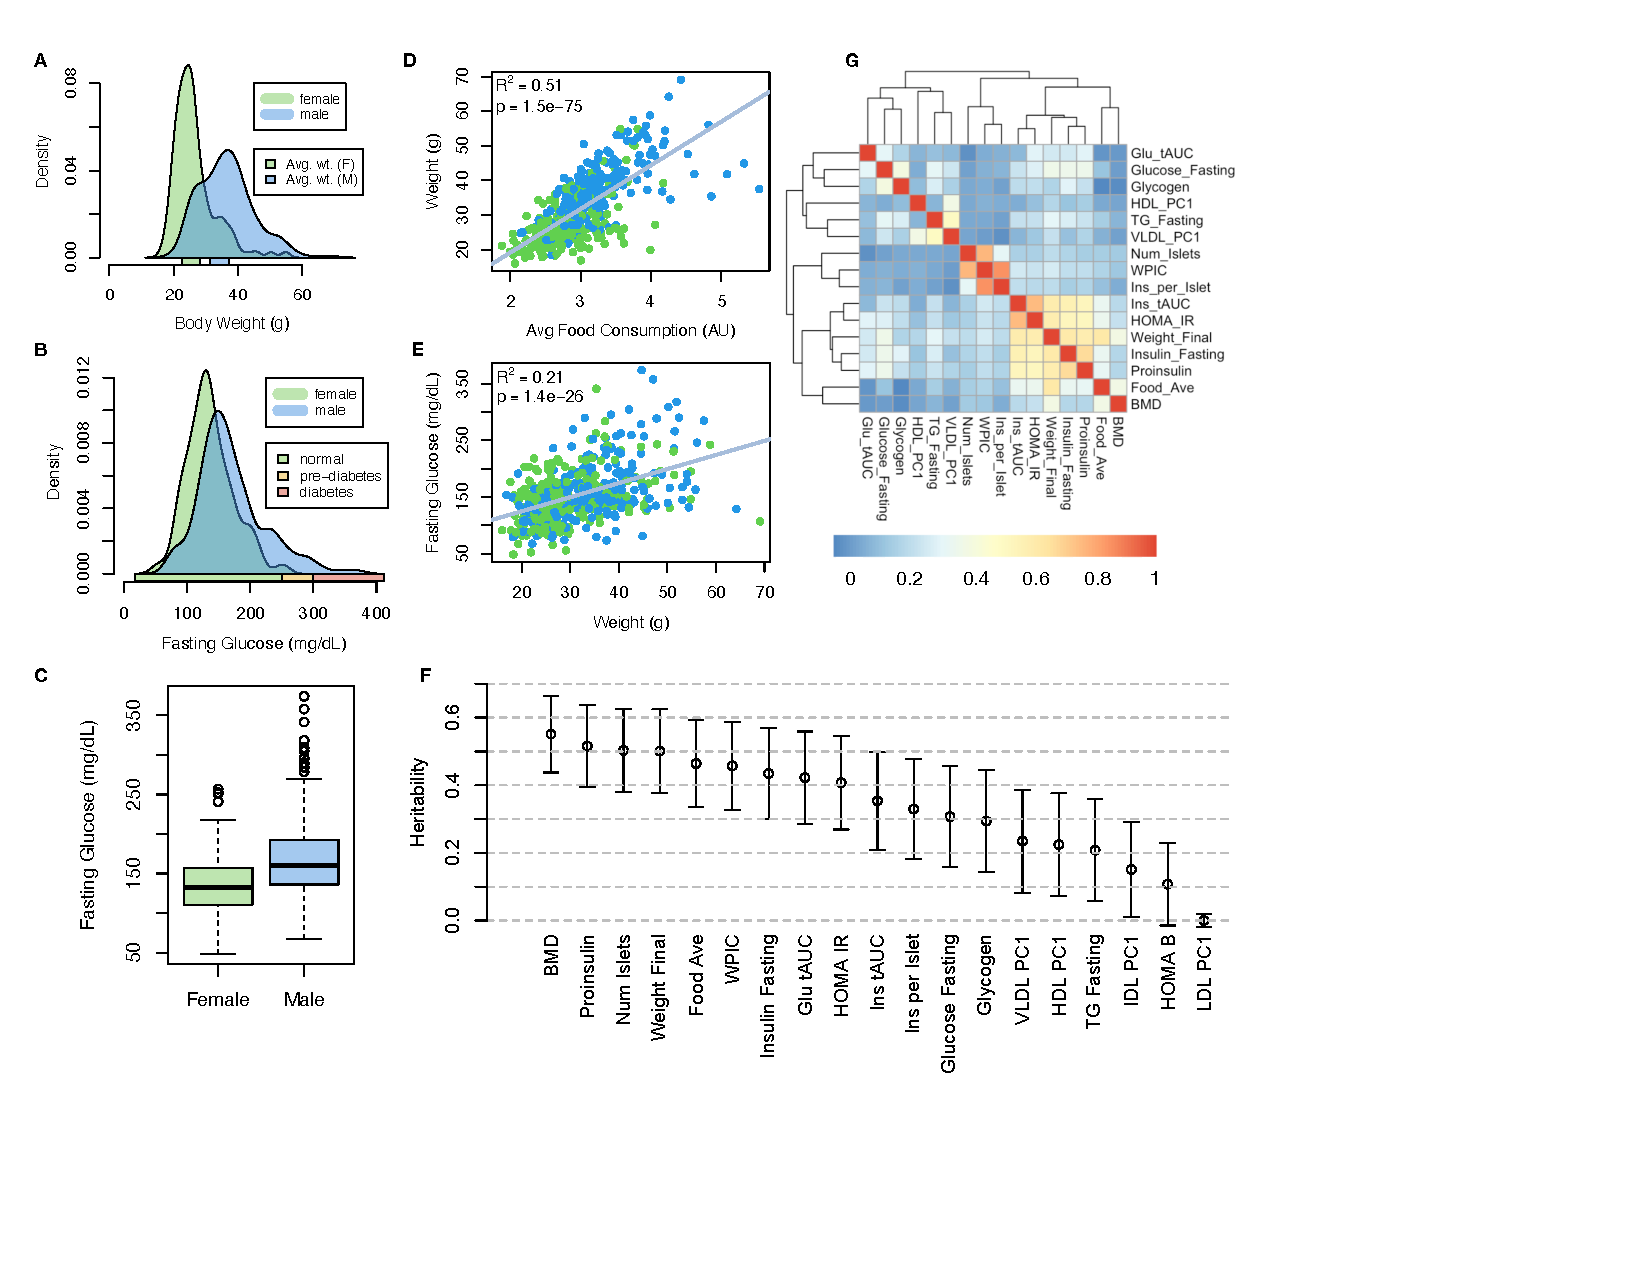
\includegraphics[width=\textwidth]{Figures/Fig1_trait_overview.pdf}
\caption{Clinical overview. \textbf{A.} Distributions of final body 
weight in female (green) and male (blue) diversity outbred mice.
The average B6 female and male adult weights at 24 weeks of 
age are indicated by green and blue bars respectively on the 
$x$-axis. \textbf{B.} Distributions of fasting glucose in female 
(green) and male (blue) DO mice. Normal (green), pre-diabetic
(yellow), and diabetic (red) fasting glucose ranges for mice are 
shown by colored bars along the $x$-axis. \textbf{C.} Males 
(blue $n = 242$) had higher fasting blood glucose on average 
(mean = 170.0 mg/dL) than females (green $n = 240$, 
mean = 136) (two-sided Welch's t test: $t = 8.02$, 
df = 428.9, 95\% CI of difference = 25.4 to 42.0 mg/dL; 
$p = 1.05\times10^{-14}$). Lines in boxes 
correspond to the median; lower and upper edges of 
boxes indicate the first and third quartiles; whiskers 
indicate the first and third quartiles $\pm$ 1.5 times
the interquartile range; dots indicate outliers beyond 1.5 times
the interquartile range. \textbf{D.} The relationship between 
food consumption and body weight for female (green) and 
male (blue) DO mice. (Linear regression 
$R^2 = 0.51$;  beta coefficient = $12.6\pm0.57$ 
standard error; $t = 22.2$; $p < 2.2^{-16}$). \textbf{E.} 
Relationship between body weight and fasting glucose for 
female (green) and male (blue) DO mice. (Linear regression 
$R^2 = 0.21$; beta coefficient = $2.49\pm 0.22$ 
standard error; $t = 11.34$; $p < 2.2^{-16}$). In D and E,
blue lines show line of best fit. \textbf{F.} Data 
presented are heritability estimates for each physiological trait. 
Bars show standard error of each estimate. The number of animals 
used in each estimate is shown in parentheses after each trait name. 
\textbf{G.} Correlation structure between pairs of physiological 
traits. The upper and lower triangle show the Pearson correlation 
coefficients ($r$) between LOD traces of trait pairs (blue) and trait 
pairs (purple) respectively. The diagonal (orange) shows the estimated 
heritability of each trait. BMD - bone mineral density, WPIC - whole 
pancreas insulin content, Glu tAUC - glucose total area under the 
curve, HOMA IR - homeostatic measurement of insulin resistance, 
HOMA B - homeostatic measure of beta cell health, VLDL - very 
low-density lipoprotein, LDL - low-density lipoprotein, IDL - intermediate 
density lipoprotein, HDL - high-density lipoprotein, TG - triglyceride. 
Source data are provided as a Source Data file.
}
\label{fig:trait_overview}
\end{figure}

\begin{figure}[ht!]
%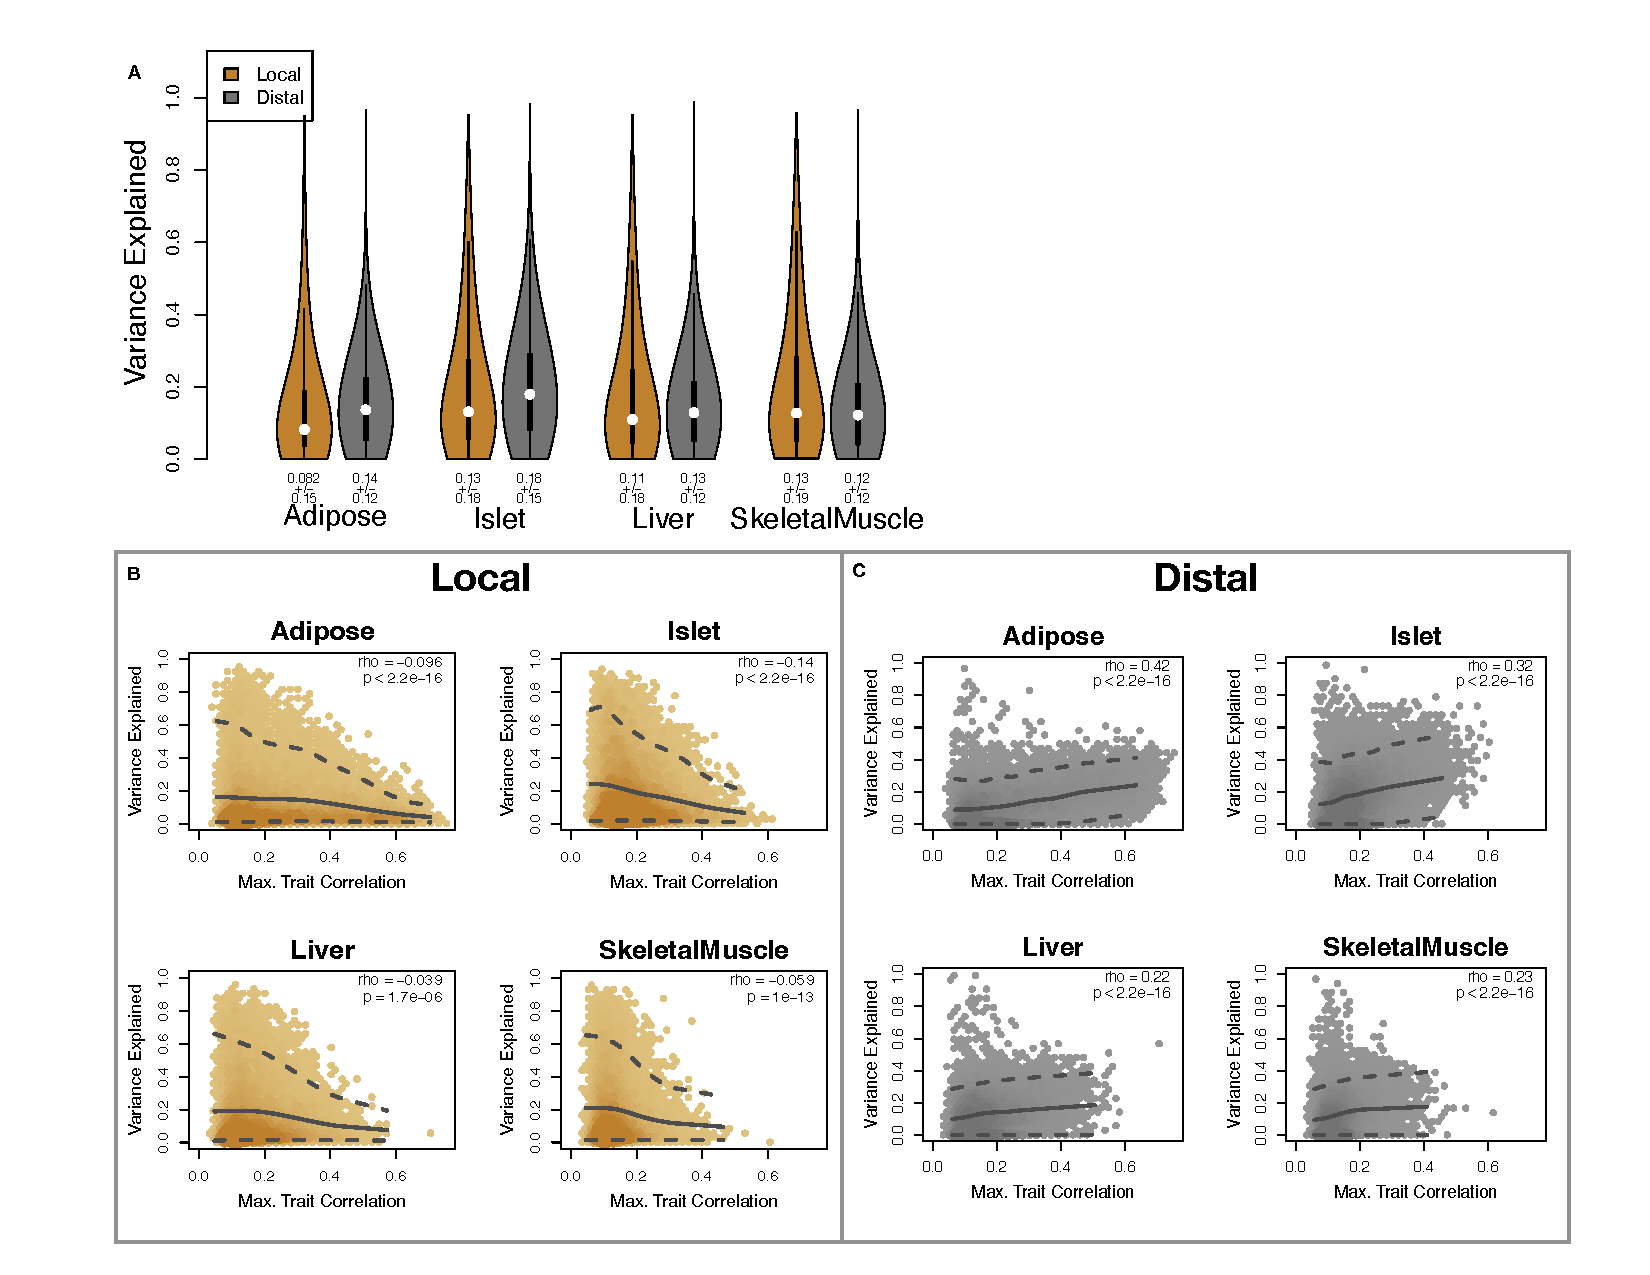
\includegraphics[width=\textwidth]{Figures/Fig2_motivation.pdf} 
\caption{Transcript heritability and trait relevance. 
\textbf{A.} Distributions of local (brown) and distal (gray) 
heritability of transcripts across the four tissues. Overall 
local and distal factors contribute equally to transcript 
heritability. Each distribution contains 14102 transcripts. 
Numbers below distributions indicate the median and 
standard deviation of each. \textbf{B.} local (brown) and 
\textbf{C.} distal (gray) heritability and trait relevance across 
all four tissues. Here trait relevance is defined as the maximum 
correlation between the transcript and all traits. The upper 
and lower dashed line in each panel show the 95th and 5th 
percentile correlation respectively. The solid line shows the 
mean trait correlation in transcripts with increasing variance 
explained either locally (B) or distally (C). Transcripts that are 
highly correlated with traits tend to have low local heritability 
and high distal heritability. All $p$ values from Spearman rank
correlation tests are two-sided. No adjustments were made 
for multiple comparisons. Source data are provided as a Source 
Data file.
}
\label{fig:motivation}
\end{figure}

\begin{figure}[ht!]
%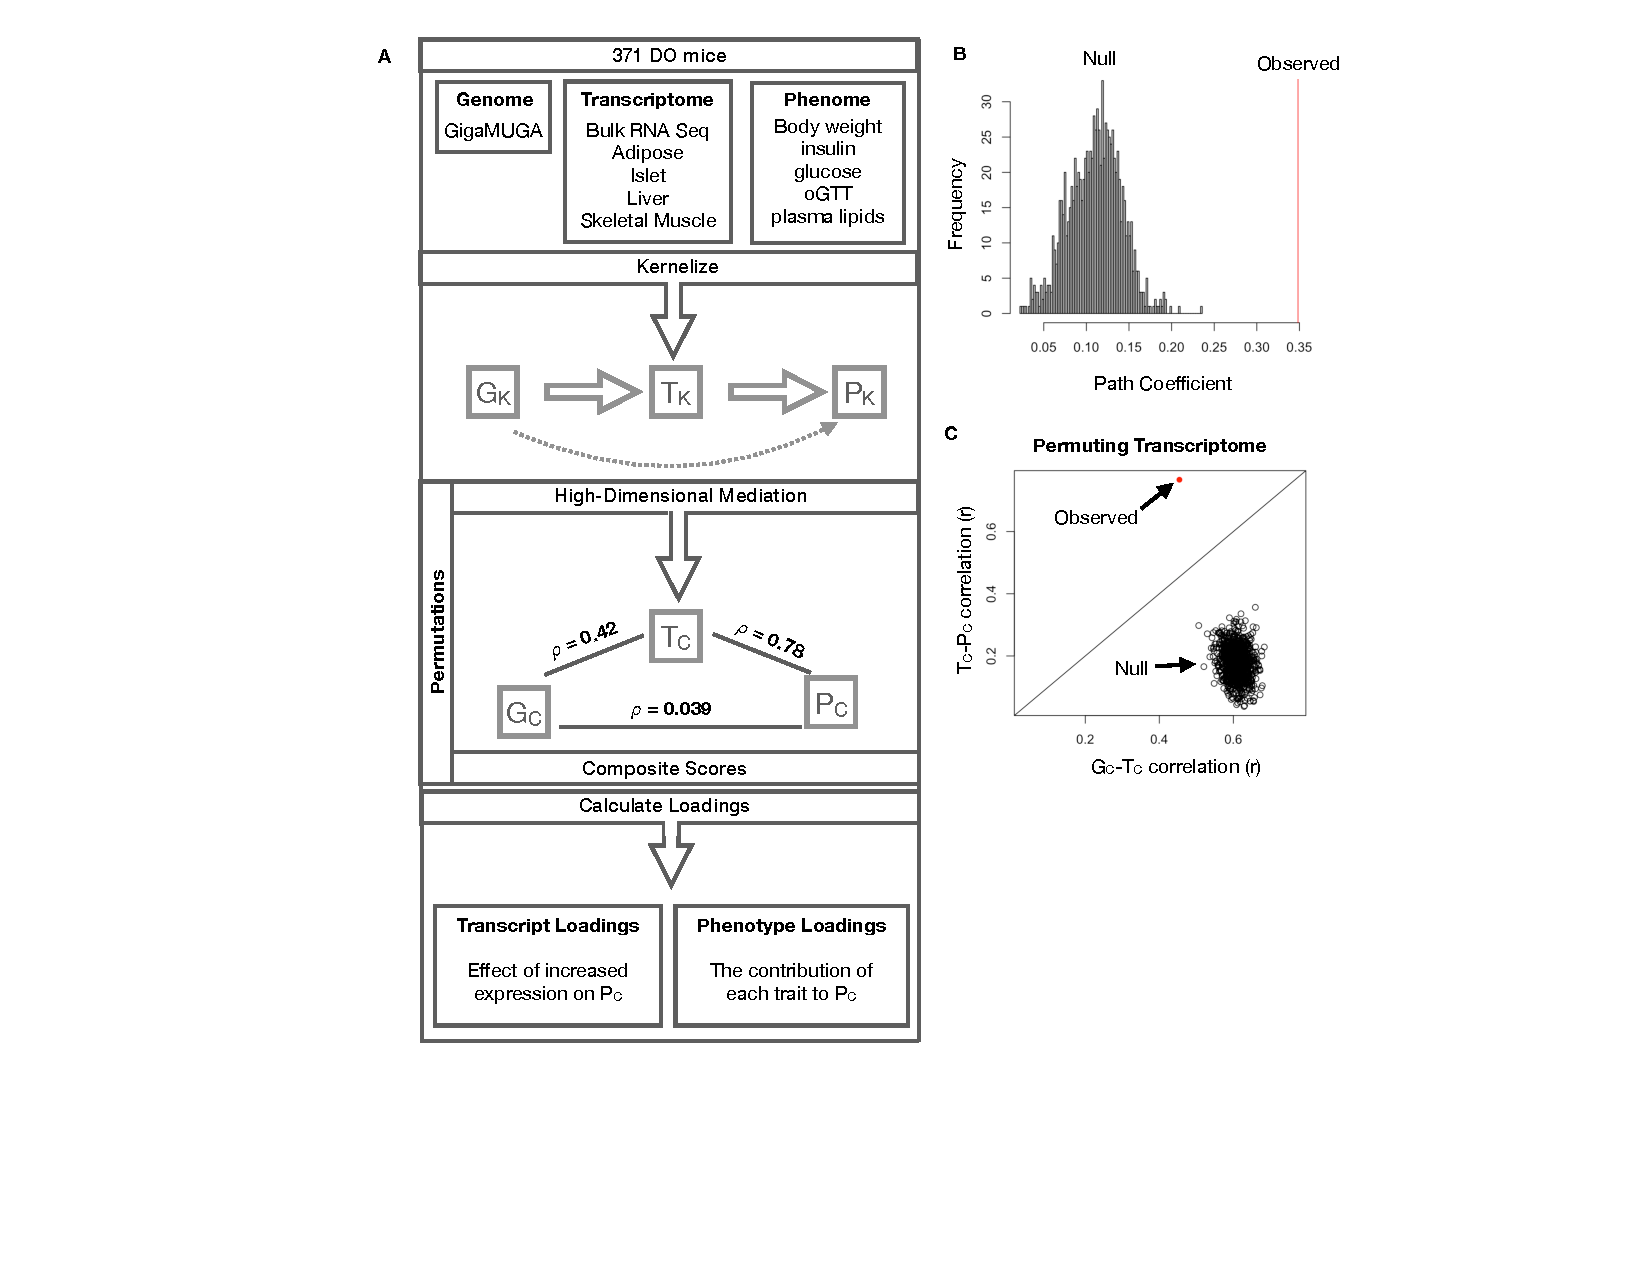
\includegraphics[width=5in]{Figures/Fig3_workflow.pdf} 
\caption{High-dimensional mediation. \textbf{A.} Workflow 
indicating major steps of high-dimensional mediation. The 
genotype, transcriptome, and phenotype matrices were 
kernelized to yield single matrices representing the 
relationships between all individuals for each data modality 
($G_K$ = genome kernel, $T_K$ = transcriptome kernel; 
$P_K$ = phenome kernel). High-dimensional mediation 
was applied to these matrices to maximize the direct path 
$G \rightarrow T \rightarrow P$, the mediating pathway 
(arrows), while simultaneously minimizing the direct $G 
\rightarrow P$ pathway (dotted line). The composite 
vectors that resulted from high-dimensional mediation 
were $G_c$, $T_C$, and $P_C$. The partial correlations 
$\rho$ between these vectors indicated perfect mediation. 
Transcript and trait loadings were calculated as described 
in the methods. \textbf{B.} The null distribution of the path 
coefficient derived from 10,000 permutations. Comparisons 
are shown to the observed path coefficient (red) the path 
coefficient using a distal-only model (gray) and the path 
coefficient using the local-only model (brown). \textbf{C.} 
The null distribution of the $G_C$-$T_C$ correlation vs. 
the $T_C$-$P_C$ correlation. Comparisons are shown 
to the observed values (red), and those derived from the 
distal-only model (gray) and the local-only model (brown).
Source data are provided as a Source Data file.
}
\label{fig:workflow}
\end{figure}

\begin{figure}[ht!]
%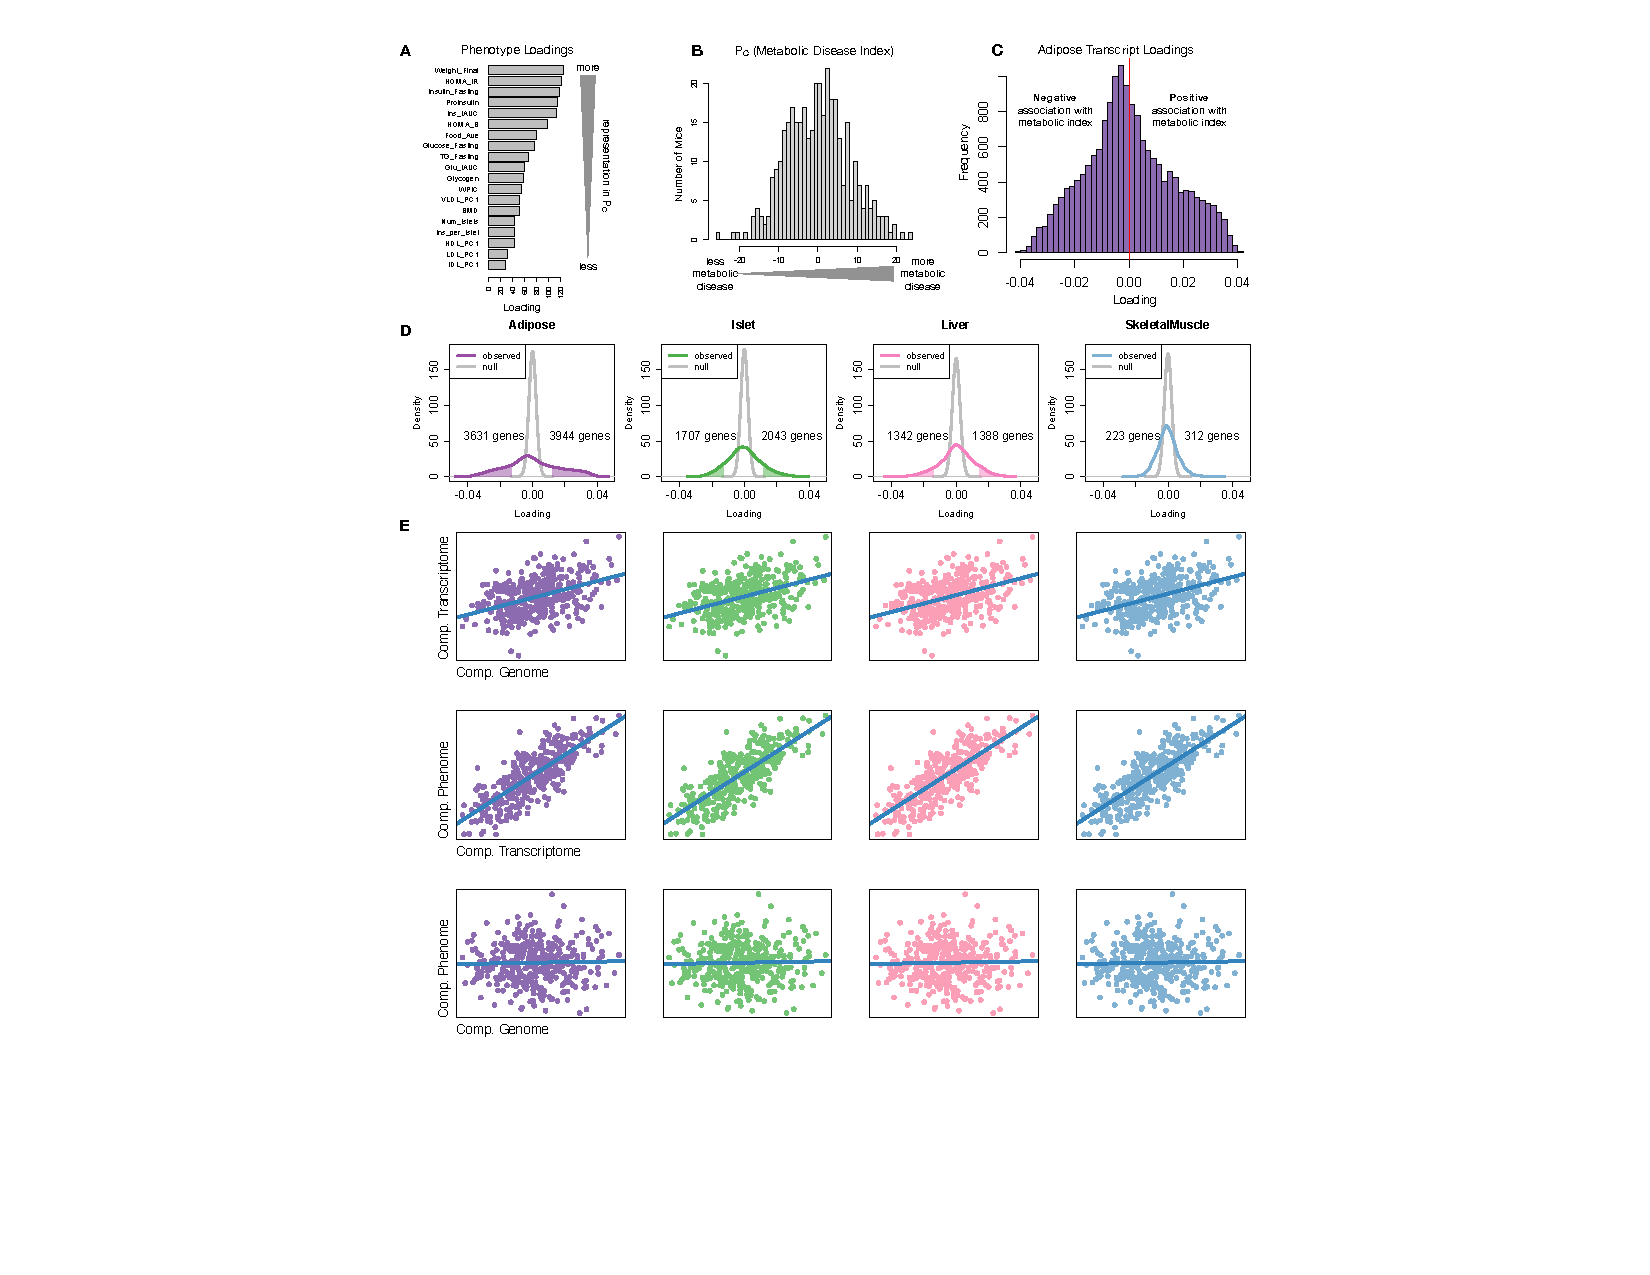
\includegraphics[width=\textwidth]{Figures/Fig4_interpretation.pdf} 
\caption{Interpretation of loadings. \textbf{A.} Loadings across traits. 
Body weight and insulin resistance contributed the most 
to the composite trait. \textbf{B.} Phenotype scores across 
individuals. Individuals with large positive phenotype scores 
had higher body weight and insulin resistance than average. 
Individuals with large negative phenotype scores had lower 
body weight and insulin resistance than average. \textbf{C.} 
Distribution of transcript loadings in adipose tissue (purple). 
For transcripts with large positive loadings, higher expression 
was associated with higher phenotype scores. For transcripts 
with large negative loadings, higher expression was associated 
with lower phenotype scores. \textbf{D.} Distributions of loadings 
across tissues compared to null distributions. Shaded areas 
represent loadings that were more extreme than the null 
distribution. Numbers indicate how many transcripts had loadings 
above and below the extremes of the null. Transcripts in adipose 
tissue (purple) had the most extreme loadings indicating 
that transcripts in adipose tissue were the best mediators of the 
genetic effects on body weight and insulin resistance. \textbf{E.} 
Scatter plots showing correlations between composite vectors for 
the genome ($G_C$), the transcriptome ($T_C$), and the phenome 
($P_C$). The $G_C$ - $T_C$ association was significant 
(Linear regression $R^2 = 0.18$;  beta coefficient = $7.8\pm0.86$ 
standard error; $t = 9.03$; $p < 2.2^{-16}$). The $T_C$ - $P_C$ 
association was significant (Linear regression $R^2 = 0.62$;  
beta coefficient = $3.1\pm0.13$ standard error; $t = 24.4$; 
$p < 2.2^{-16}$). There is no association between $G_C$ and $P_C$
(Linear regression $R^2 = 7.1\times10^{4}$;  beta coefficient = 
$2.0\pm3.8$ standard error; $t = 0.51$; $p = 0.61$). This correlation 
structure is consistent with perfect mediation. Blue lines show
lines of best fit. Source data are provided as a Source Data file.
}
\label{fig:interpretation}
\end{figure}

\begin{figure}[ht!]
%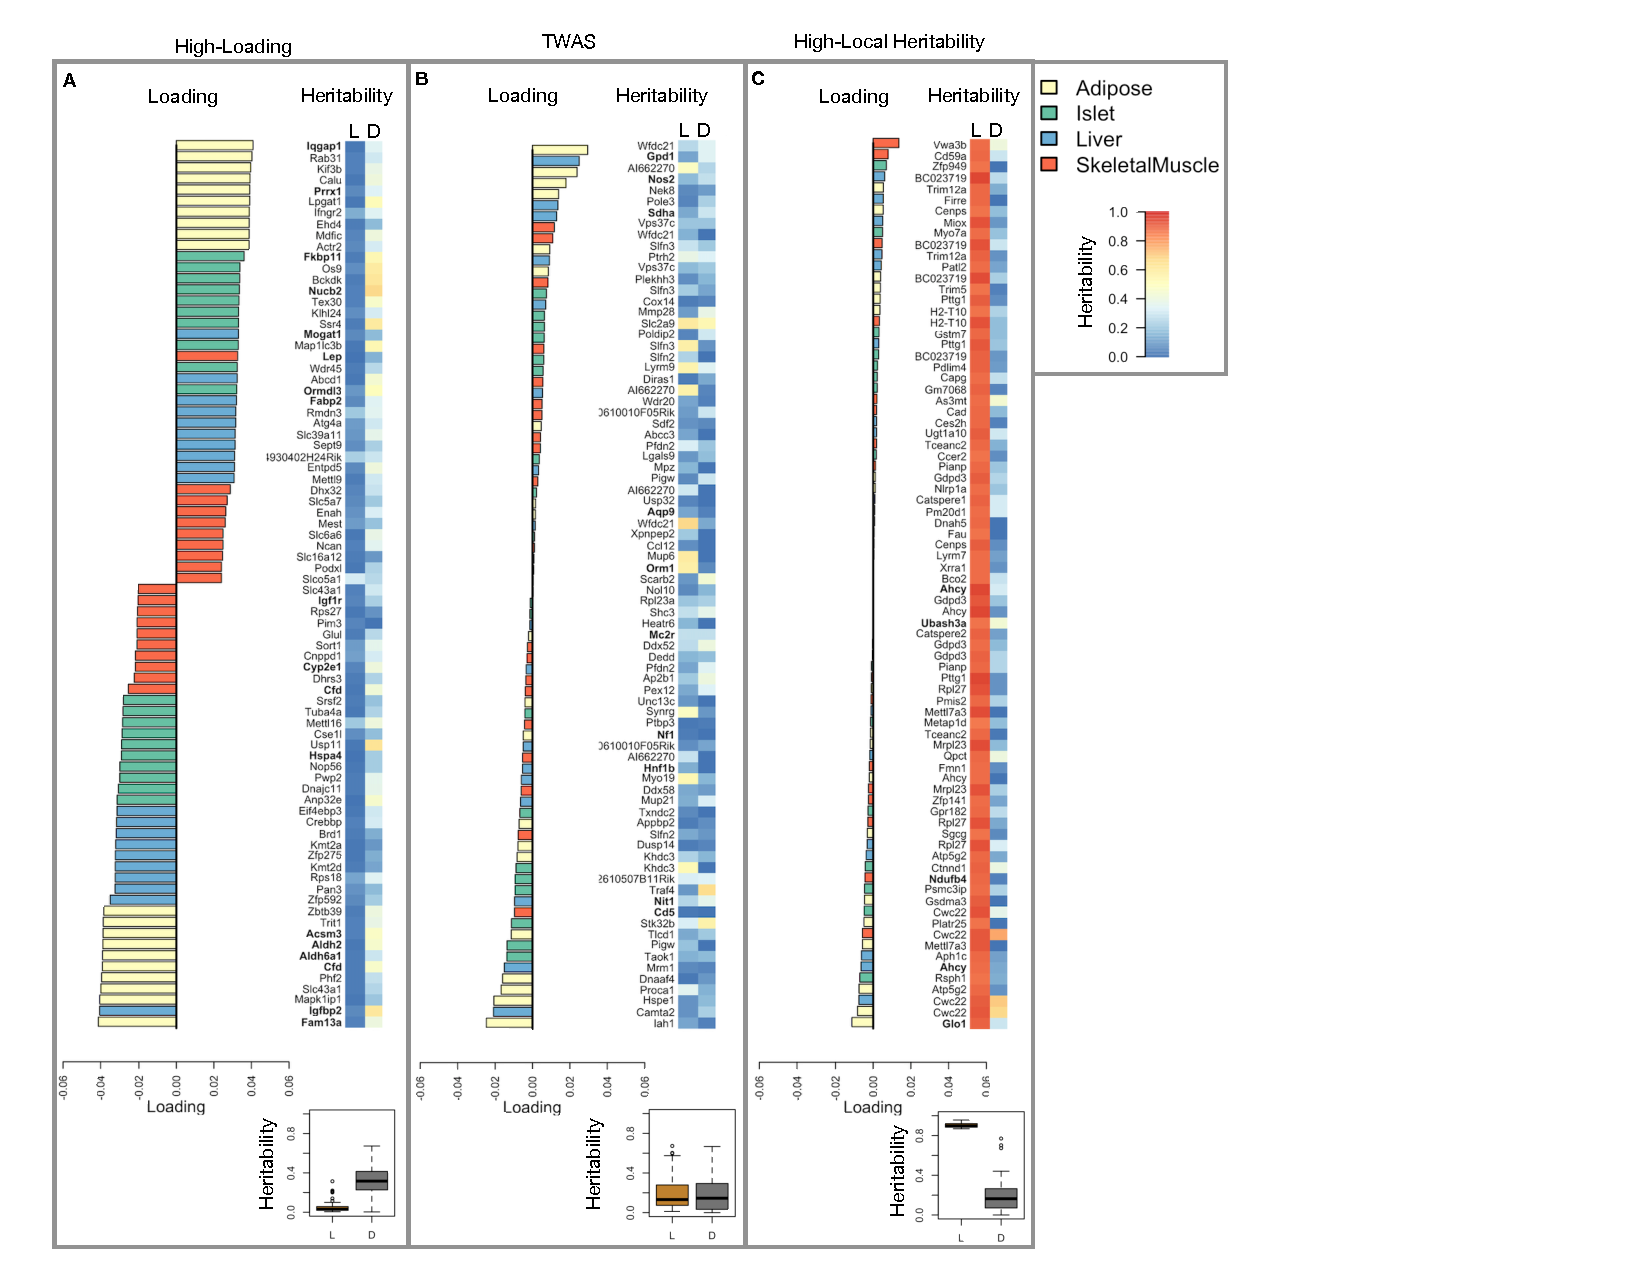
\includegraphics[width=\textwidth]{Figures/Fig5_loading_heritability.pdf} 
\caption{Transcripts with high loadings have high distal heritability 
and literature support. Each panel has a bar plot showing 
the loadings of transcripts selected by different criteria. 
Bar color indicates the tissue of origin. The heat map 
shows the local (L - left) and distal (D - right) heritability 
of each transcript. \textbf{A.} Loadings for the 10 
transcripts with the largest positive loadings and the 10 
transcripts with the largest negative loadings for each tissue. 
Mean distal heritability (31.8\%) was significantly higher than 
mean local heritability (5\%) (two-sided Welch's 
t-test $t = 16.4$; df = 100.2; difference 95\% CI = 0.24 to 
0.30; $p < 2.2^{-16}$). \textbf{B.} Loadings of TWAS 
candidates with the 10 largest positive correlations with 
traits and the largest negative correlations with traits across 
all four tissues. Mean local (15\%) and distal (20\%) heritability
were not significantly different for this group of transcripts 
(two-sided Welch's t-test $t = 1.9$; df = 151.7; difference 95\% 
CI = -0.002 to 0.1; $p = 0.77$). \textbf{C.} The transcripts 
with the largest local heritability (top 20) across all four 
tissues. Mean local heritability (90\%) was significantly higher 
than mean distal heritability (15\%) of these genes 
(two-sided Welch's $t = 45.0$; df = 82.0; difference 95\% 
CI = 0.72 to 0.78; $p < 2.2^{-16}$). Lines in boxes correspond 
to the median; lower and upper edges of boxes indicate the 
first and third quartiles; whiskers indicate the first and 
third quartiles $\pm$ 1.5 times the interquartile range; dots 
indicate outliers beyond 1.5 times the interquartile range. All 
$p$ values derived from two-sided Welch's t-test and are 
not adjusted for multiple comparisons. Source data are 
provided as a Source Data file.
}
\label{fig:loading_heritability}
\end{figure}

\begin{figure}[ht!]
%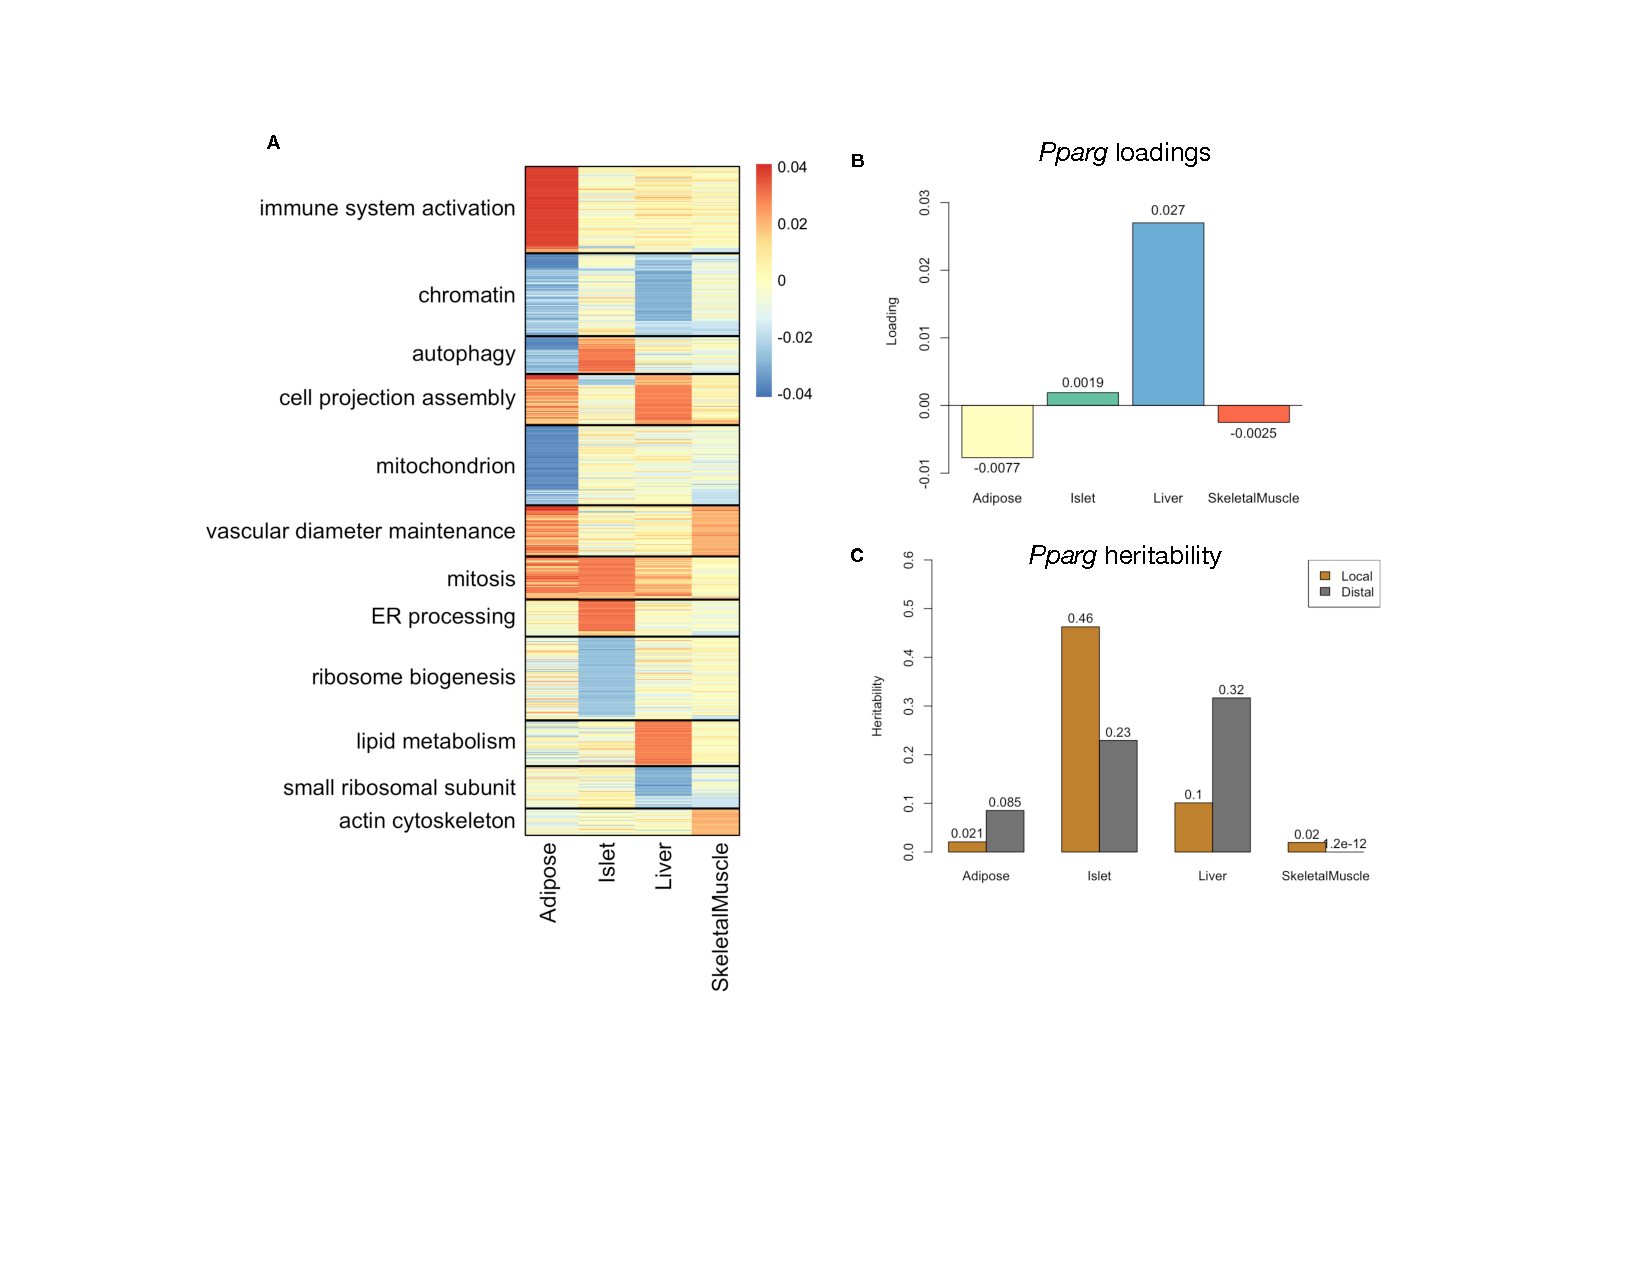
\includegraphics[width=\textwidth]{Figures/Fig6_TOA.pdf} 
\caption{Tissue-specific transcriptional programs are 
associated with obesity and insulin resistance. \textbf{A} 
Heat map showing the loadings of all transcripts with 
loadings greater than 2.5 standard deviations from the 
mean in any tissue. The heat map was clustered using 
$k$ medoid clustering. Functional enrichments of each 
cluster are indicated along the left margin. \textbf{B} 
Loadings for \textit{Pparg} in different tissues indicated 
by color. \textbf{C} Local (brown) and distal (gray) of 
\textit{Pparg} expression in different tissues. Source data 
are provided as a Source Data file.
}
\label{fig:toa}
\end{figure}

\begin{figure}[ht!]
%\includegraphics[width=\textwidth]{Figures/Fig7_CC_Prediction.pdf} 
\caption{Transcription, but not local genotype, predicts 
phenotype in the CC-RIX. \textbf{A.} Workflow showing 
procedure for translating HDM results to an independent 
population of mice. \textbf{B.} Relationships between the 
predicted metabolic disease index (MDI) and the mean
of the rankZ normalized body weight. In this column,
MDI was derived from measured transcripts. Adipose - 
$R^2 = 0.60$;  beta coefficient = $0.89\pm0.17$ 
standard error; $t = 5.21$; $p = 5.9\times10^{-5}$.
Liver - $R^2 = 0.35$;  beta coefficient = $1.1\pm0.34$ 
standard error; $t = 3.1$; $p = 6.4\times10^{-3}$.
Muscle - $R^2 = 0.29$;  beta coefficient = $0.64\pm0.24$ 
standard error; $t = 2.7$; $p = 0.014$.
\textbf{C.} In this column, MDI was derived from 
transcripts imputed from local genotype. Adipose - 
$R^2 = 8.0\times10^{-4}$;  beta coefficient = $-0.2\pm0.16$ 
standard error; $t = -0.12$; $p = 0.91$.
Liver - $R^2 = 0.035$;  beta coefficient = $0.13\pm0.16$ 
standard error; $t = 0.81$; $p = 0.43$.
Muscle - $R^2 = 0.079$;  beta coefficient = $0.19\pm0.16$ 
standard error; $t = 1.24$; $p = 0.23$.
Gray boxes indicate measured quantities and blue boxes 
indicate calculated quantities. G - genome; T - transcriptome; 
P - phenome (here MDI). The dots in each panel represent 
individual CC-RIX strains. Each strain was represented 
by between 19 and 24 individuals. The gray lines show 
the standard deviation of mean body weight for the 
strain. Source data are provided as a Source Data 
file.
}
\label{fig:cc_prediction}
\end{figure}

\begin{figure}[ht!]
%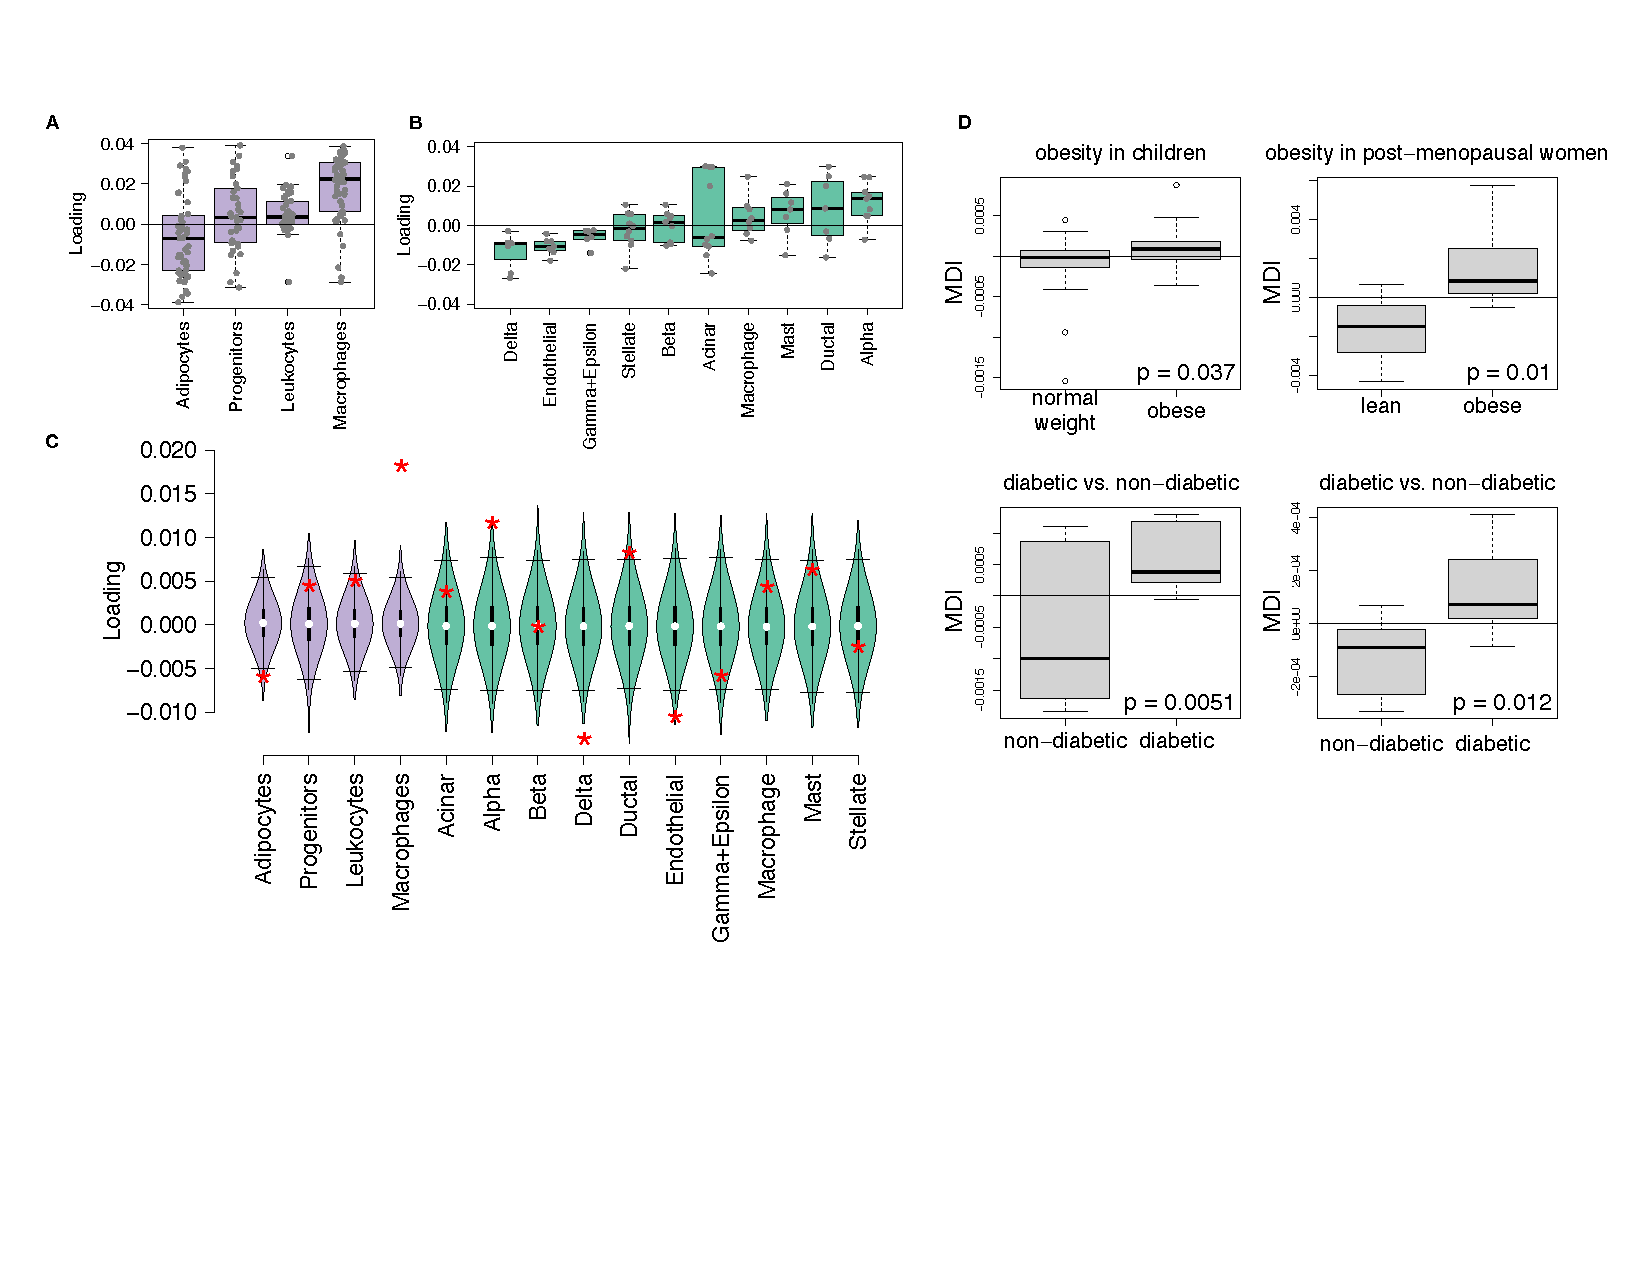
\includegraphics[width=\textwidth]{Figures/Fig8_Human_Translation.pdf} 
\caption{HDM results translate to humans. \textbf{A.} Distribution of 
loadings for cell-type-specific transcripts in adipose tissue
(purple). Numbers in parentheses indicate the number of 
transcripts in each group. \textbf{B.} Distribution of loadings 
for cell-type-specific transcripts in pancreatic islets (green). 
Each box in this panel represents 10 transcripts. \textbf{C.} 
Null distributions from 10,000 permutations for the mean 
loading of randomly selected transcripts in each cell type 
compared with the observed mean loading of each group 
of transcripts (red asterisk). Violin plot colors indicate the 
tissue of each cell type and match panels A and B 
(purple = adipose; green = islet) \textbf{D.} Predictions of 
metabolic phenotypes in four adipose transcription data 
sets downloaded from GEO. In each study the obese/diabetic 
patients were predicted to have greater metabolic disease 
than the lean/non-diabetic patients based on the HDM 
results from DO mice. Lines in boxes correspond to the 
median; lower and upper edges of boxes indicate the 
first and third quartiles; whiskers indicate either the minimum
and maximum values if no outliers, or the first and third quartiles 
$\pm$ 1.5 times the interquartile range if there are outliers; 
dots indicate outliers beyond 1.5 times the interquartile range. 
The number of patients in each group is indicated by numbers 
in parentheses. The $p$ values reported are derived from two-sided
Welch's t tests. No adjustments were made for multiple comparisons. 
Source data are provided as a Source Data file.
}
\label{fig:human_translation}
\end{figure}

\end{document}
